\documentclass{article} % For LaTeX2e

%STANDARD PREAMBLE
%https://tex.stackexchange.com/questions/68821/is-it-possible-to-create-a-latex-preamble-header
\usepackage{/Users/mwojno01/Research/Learning/latex_preamble/preamble}

%%% 
% SPECIFIC TO THIS DOCUMENT
%%%

% SIGMA-FIELDS 
% Sigma fields (text)
\renewcommand{\sf}{$\sigma$-field}
\newcommand{\sfs}{$\sigma$-fields}


% SET FUNCTIONS 
%Finitely additive set functions
\newcommand{\fasf}{\tilde{\mu}_0}
% Signed measure
\newcommand{\signedmu}{\wt{\mu}}

% RATIONALS
\renewcommand{\Q}{\mathbb{Q}}
\begin{document}


\title{Notes on Probability and Measure Theory} 
\maketitle
\setcounter{tocdepth}{2}
\tableofcontents
\newpage 

\section{Overview}

\subsection{References}
The primary reference here is \cite{ash2000probability}.   The book is wonderful for statistical machine learning – it is rigorous,  but also accessible (prerequisites are undergrad-level real analysis and mathematical probability).  Most importantly, it is structured to build towards the kinds of applications in probability that we care about.   (A point of contrast would be a book like that of Stein and Shakarchi, which tends to dwell heavily on things that are of higher interest to pure mathematicians –- long existence proofs, Cantor sets and fractals, etc.) 

 Unless otherwise specified, all references to the ``text" refers to this textbook.  Likewise the symbol $\S$ refers to a Section of that textbook.
 
\subsection{Motivation for topic} \label{sec:motivation_for_topic}

What are some motivations for measure theory?

\begin{itemize}
\item Measure theory underpins some of the most interesting research in Bayesian statistics and probabilistic machine learning (see work from Stephen G. Walker, Michael Jordan, Tamara Broderick, David Dunson, and so on).   Thus, fluency with measure theory opens doors to a higher level of research consumption. 
\item Measure theory underpins research on stochastic processes (as used in Bayesian nonparametrics) and stochastic differential equations (useful for continuous-time time series models, a current topic of active research interest in machine learning). 
\item Measure theory is convenient in unifying various kinds of random variables.\footnote{For example, it allows one to work with discrete and absolutely continuous random variables in a unified way.  For example, the exponential family includes both types of random variables.}
\item Lebesgue integration provide nice limit theorems, e.g. clarifying when one can interchange integrals and limits (such as derivatives).   
\item Lesbesgue integrals can be seen as the completion of Reimann integrals (in the same way that the real numbers complete the rationals).
\item Abstract Lebesgue integration allows one to integrate over spaces more general than the reals. 

\end{itemize}



\subsection{Motivation for notes}

It is hard to beat directly consulting a textbook (such as \cite{ash2000probability}) written by a seasoned mathematician who is an excellent pedagogue.

However, we have created these notes nonetheless in an attempt to support lecture and/or discussion on that textbook.   With that goal in mind, we:
\begin{itemize}
\item Curate the text.\footnote{We highlight some of the main themes (and cores of proofs), offloading additional detail to the text.} 
\item Provide additional detail in proofs.
\item Format the presentation to encourage easier absorption.\footnote{E.g., we exploit space to organize the presentation, whereas a textbook will often provide proofs in paragraph form}
\item Add remarks to illustrate the utility of theorems and draw connections between them.
\item Add sketches to support intuition.
\item Incorporate supporting material, such as additional examples, from homework problems and outside sources.\footnote{This will happen increasingly often as the notes evolve.}
\end{itemize}


%We begin with a discussion of $\sigma$-fields, which are the domains of probability measures, and measures more generally.  As it turns out, measures cannot be defined on all subsets of many spaces that we would like to deal with. For instance, consider Proposition 1.2.6 of \cite{rosenthal2006first} which asserts the existence of non-measurable sets for the uniform distribution.  In particular, there is no definition of $P(A)$ that is defined for all subsets $A \subseteq [0,1]$ satisfying all three conditions below



\section{$\S$ 1.1: Some notes on set theory}

\subsection{Limits of sequences of sets}

\begin{definition}
The \textbf{upper limit} of a sequence of sets is given by
\[ \lim\sup A_n := \bigcap_{n=1}^\infty \bigcup_{k \geq n} A_k \]
Alternatively,
\[ x \in \lim\sup A_n \text{ iff } x \in A_n \text{ for infinitely many } n \]
\end{definition}

\begin{definition}
The \textbf{lower limit} of a sequence of sets is given by
\[ \lim\inf A_n := \bigcup_{n=1}^\infty \bigcap_{k \geq n} A_k \]
Alternatively,
\[ x \in \lim\inf A_n \text{ iff } x \in A_n \text{ eventually ( for all but finitely many $n$ ) } \]
\end{definition}

\begin{figure}
\centering 
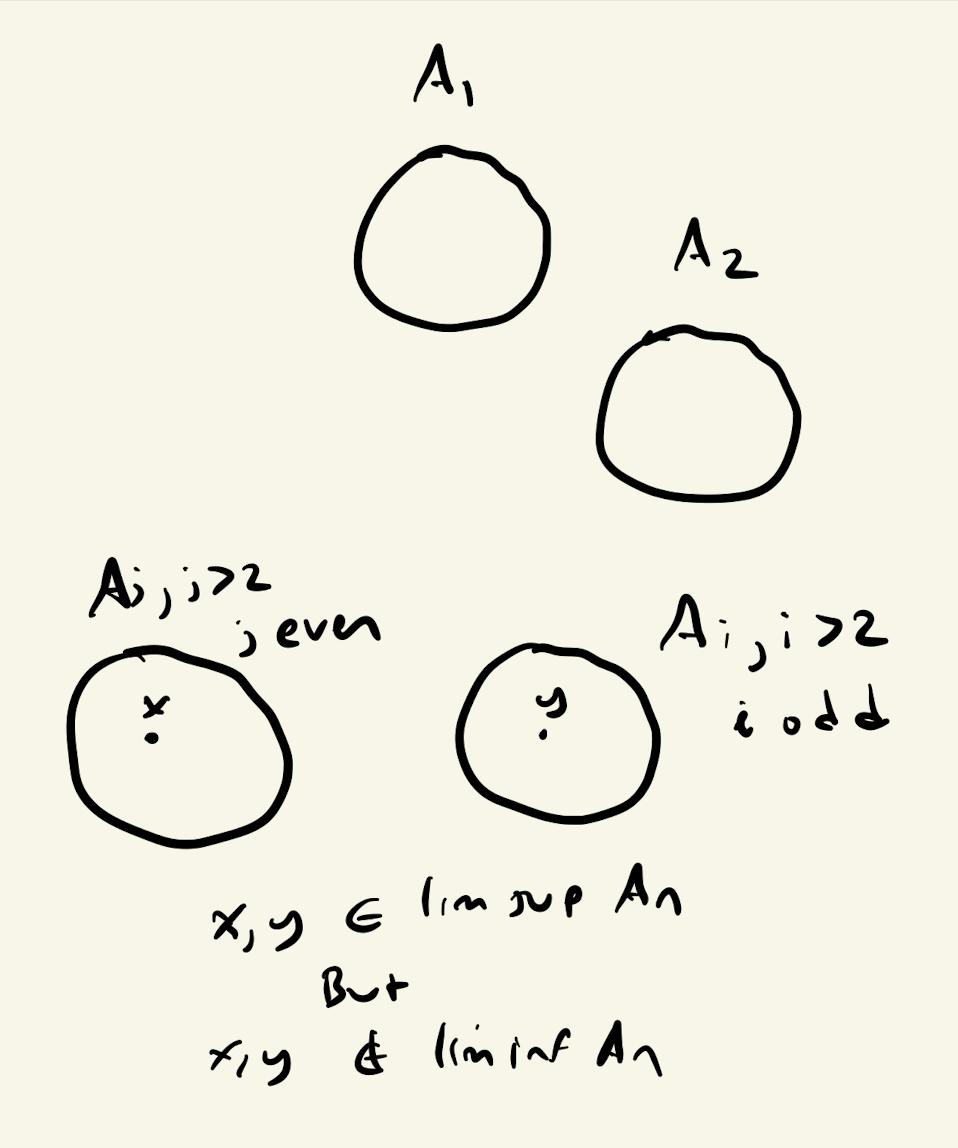
\includegraphics[width=.5\textwidth]{images/limsup_and_liminf}	
\caption{A sequence of sets with empty lower limit and non-empty upper limit.}
\end{figure}

\begin{discussion}
Discuss why the two characterizations of upper limit and lower limit are equivalent.	
\end{discussion}

\begin{definition}
If $\lim\inf A_n = \lim\sup A_n = A$, then A is called the \textbf{limit} of the sequence $A_1, A_2, ...$. 
\end{definition}

Now we present a particular kind of limit that will be useful when we discuss continuity of measure. 

\begin{definition}
If $A_1 \subset A_2 \subset ...$ and $\cup_{n=1}^\infty A_n = A$, we say that the $A_n$ form a \textbf{increasing} sequence of sets with limit $A$ or that the $A_n$ increase to $A$; we write $A_n \uparrow A$.  If $A_1 \supset A_2 \supset ... $ and  	$\cap_{n=1}^\infty A_n = A$, we say that the $A_n$ form a \textbf{decreasing} sequence of sets with limit $A$ or that the $A_n$ decrease to $A$; we write $A_n \downarrow A$.
\end{definition}


\begin{figure}[h!]
\centering 
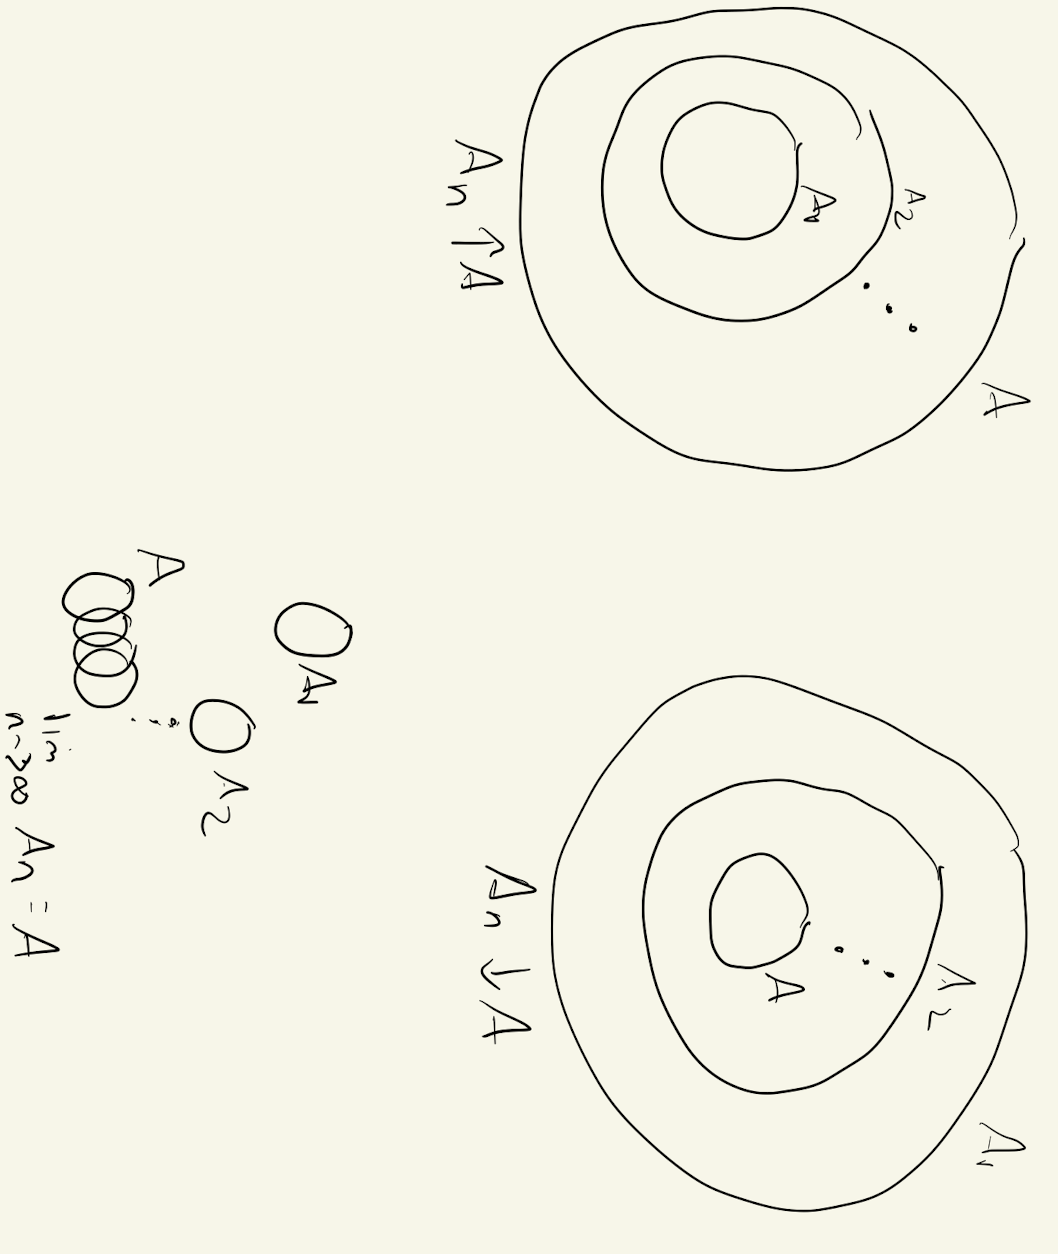
\includegraphics[width=.5\textwidth, angle=90]{images/increasing_and_decreasing_sequences}
\caption{An increasing and decreasing sequence of sets, followed by a sequence of sets which is neither, but which has a limit.}
\label{fig:increasing_and_decreasing_limits_of_sets}
\end{figure}

One can verify that this definition is consistent with the definition of limits, i.e.
\[  \text{If } A_n \uparrow A \text{ or } A_n \downarrow A \text{ then } \lim\inf A_n = \lim\sup A_n = A.\]

As shown in Figure \ref{fig:increasing_and_decreasing_limits_of_sets}, limits of increasing and decreasing sequences are very special kinds of limits.


\subsection{Representing unions as disjoint unions} \label{sec:representing_unions_as_disjoint_unions}
 
\begin{remark}
If $A_1,A_2,...$ are subsets of some set $\Omega$, then
\begin{align*} 
\bigcup_{n=1}^\infty A_n = \bigcupdot_{n=1}^\infty \bigg(A_n \cap A_{n-1}^c \cap ... \cap A_1^c \bigg) 	
\labelit \label{eqn:union_as_disjoint_union}
\end{align*}

In other words, any union can be re-represented as a disjoint union. This is useful because measures are countably additive on disjoint sets, so we prefer to work with collections of disjoint sets.
\label{rk:rerepresenting_unions_as_disjoint_unions}
\end{remark}

\begin{remark}
If $A_n \uparrow A$, then \eqref{eqn:union_as_disjoint_union} becomes
\begin{align*}
	\bigcup_{n=1}^\infty A_n = \bigcupdot_{n=1}^\infty \bigg( A_n - A_{n-1} \bigg) 
\labelit \label{eqn:union_as_disjoint_union_for_increasing_sequences}
\end{align*}
This is because $A_{n-1} \subset A_{n}$, so $A_{n-1}^c \supset A_{n}^c$ by contraposition.	
\end{remark}

\section{$\S$ 1.2: Fields, \sfs, measures}

\subsection{$\S$ 1.2.1-1.2.2: Fields and \sfs}

Probability measures, and measures more generally, cannot be defined on all subsets of many spaces that we would like to deal with.  For instance, non-measurable sets can be shown to exist even for Lesbesgue measure on the unit interval.  Proposition 1.2.6 of \cite{rosenthal2006first} shows that there is no definition of $P(A)$ that is defined for all subsets $A \subseteq [0,1]$ satisfying all three conditions below\footnote{In Proposition \ref{prop:existence_of_set_that_is_not_lesbesgue_measurable}, we make a similar observation, along with a proof: there cannot be a measure defined on all subsets of the reals that is both translation invariant and has a finite value on all bounded intervals.}
\begin{enumerate}
\item $P([a,b]) = b-a, \quad 0 \leq a \leq b \leq 1$.	
\item $P(\bigcupdot_{n=1}^\infty A_n ) = \ds\sum_{n=1}^\infty A_n$ for $A_1, A_2, ...$ disjoint subsets of $[0,1]$.
\item $P(A \bigoplus r) = P(A), \quad 0 \leq r \leq 1$, where $A \bigoplus r$ denotes the \textit{r-shift} of $A$, i.e. 
\[ A \bigoplus r := \set{a+r : a \in A, a+r \leq 1} \cup \set{a+r-1 : a \in A, a +r >1}\]
\end{enumerate}

The solution to this problem is to define measures on a restricted domain, $\sigma$-fields.

\subsubsection{$\sigma$-fields}



%We begin with a discussion of $\sigma$-fields, which are typically the domains of probability measures, and measures more generally.\footnote{In the construction of Lesbesgue measure, Ash defines a probability measure on a field.  See 1.3.1 of \cite{ash2000probability}.}  As stated in the motivation (Section \ref{sec:motivation_for_topic}), measures cannot be defined on all subsets of many spaces that we would like to deal with. 

%\sfs\ are important because they are the domain of measures.  
%Here are some definitions.

\begin{definition}
Let $\F$ be a collection of subsets of a set $\Omega$.  Then $\F$ is called a \textbf{sigma-field} (or \textit{sigma-algebra}) if it satisfies

\begin{enumerate}[label=\alph*)]
	\item $\Omega \in \F$ 
	\item If $A \in \F$, then $A^c \in \F$.
	\item If $A_1,A_2, ... \in \F$ then $\cup_{i=1}^\infty A_i \in \F$.  
\end{enumerate}
that is, if $\Omega \in \F$ and $\F$ is closed under complementation and countable unions.
\label{def:sigma_field}	
\end{definition}

\begin{remark}
It follows that $\sigma$-fields are closed under countable intersections, since
\[ \cap_{i=1}^\infty A_i \stackrel{\text{DeMorgan's Law}}{=} \cup_{i=1}^\infty A_i^c \]	
\end{remark}

\begin{example}
$\F =\set{\emptyset, \Omega}$ is the smallest \sf\ on $\Omega$. 
\end{example}

\begin{example}
	$\F =2^\Omega$, i.e. the set of all subsets of $\Omega$, is the largest \sf\ on $\Omega$.
\end{example}

\begin{example}
If $A \in \Omega$ is non-empty, then $\F = \set{\emptyset, A, A^c, \Omega}$ is the smallest \sf\ containing $A$.
\end{example}

\begin{notation}
If $\C$ is a class of sets, the smallest \sf\ containing the sets of $\C$ is written as $\sigma(\C$).  This is sometimes called the \textit{minimal \sf\ over $C$} or the \textit{\sf\ generated by $C$}. 
\end{notation}
	
\begin{exercise}
\label{exercise:minimal_sigma_field_containing_n_subsets}
Let $A_1,...,A_n$ be subsets of $\Omega$.  Describe $\F := \sigma(\set{A_1,...,A_n})$, the smallest \sf\ containing $A_1,...,A_n$.  Also describe the number of sets in $\F$.   \textit{This is Ash's Problem 1.2.8.  We can derive the strict upper bound $|\F| \leq 2^{2^n}$. For a complete answer, see GoodNotes. }	
\end{exercise}

\begin{remark}
The gist of exercise \ref{exercise:minimal_sigma_field_containing_n_subsets} is that the collection $\set{A_1,...,A_n}$ partitions $\Omega$ into up to $M=2^N$ pieces, and the minimal sigma field contains all possible finite unions of these pieces, so has at most $2^{M}$ elements.
  
\begin{figure}[h!]
\centering 
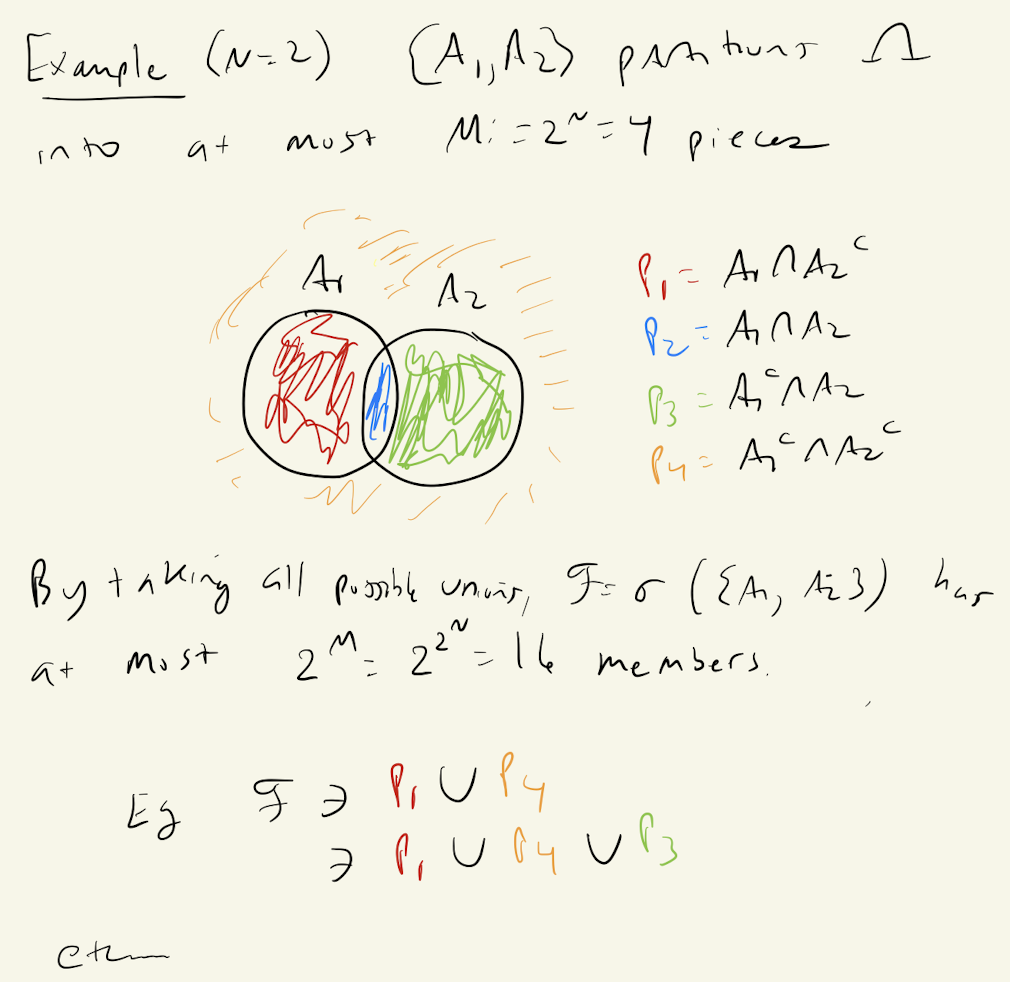
\includegraphics[width=.7\textwidth]{images/minimal_sigma_fields}
%\caption{An increasing and decreasing sequence of sets, followed by a sequence of sets which is neither, but which has a limit.}
\end{figure}

\end{remark}

\subsubsection{Fields}

Fields are more general than $\sigma$-fields.  Measures are sometimes constructed by being defined on fields, and then extended to \sfs.  Indeed, we will see this strategy with Lesbesgue measure. 

\begin{definition}
Let $\F$ be a collection of subsets of a set $\Omega$.  Then $\F$ is called a \textbf{field} (or \textit{algebra})  if satisfies Definition \ref{def:sigma_field} after replacing condition c) with

\begin{enumerate}
	\item[c')] If $A_1,...A_n \in \F$ then $\cup_{i=1}^n A_i \in \F$.
\end{enumerate}
that is, if $\Omega \in \F$ and $\F$ is closed under complementation and \textit{finite} unions.
\label{def:field}	
\end{definition}

\begin{example} What is an example of a collection that is a \textit{field}, but not a $\sigma$-\textit{field}?  

Let $\Omega=\R$ and $\F_0 = \set{\text{finite disjoint unions of right semi-closed intervals } (a,b], a \neq b}$.  Then $\F_0$ is a field, as can be easily verified.\footnote{By convention, we also count $(a, \infty)$ as right semi-closed for $-\infty\leq a < \infty$, which is necessary for the \sf\ to be closed under complements.}   

\begin{figure}[h!]
\centering
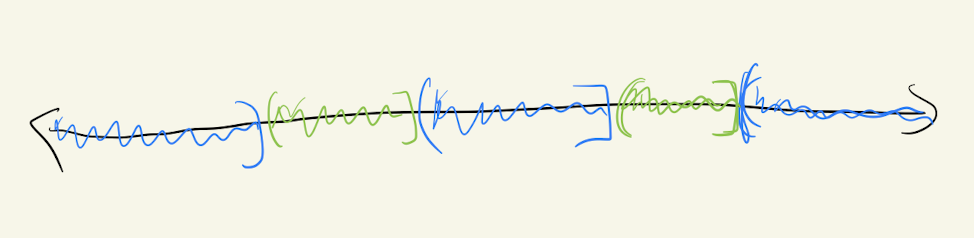
\includegraphics[width=.6\textwidth]{images/rsc_intervals}	
\end{figure}

But $\F_0$ is \underline{not} a \sf.  Note that if $A_n = (-\frac{1}{n},0]$, then $\bigcap_{n=1}^\infty A_n = \set{0}  \not\in \F_0$.
\label{ex:field_of_finite_disjoint_unions_of_rsc_intervals}
\end{example}

\begin{remark}
 If $\F$ is a field, a countable union of sets in $\F$ can be expressed as the limit of an increasing sequence of sets in $\F$, and conversely. For if $A_n \in \F$ and $A_n \uparrow A$, then A is a countable union of sets in $\F$ by definition.  Conversely, if $A = \cup_{n=1}^\infty A_n$, then set $B_N := \cup_{n=1}^N A_n$ and $B_N \uparrow A$. This shows that a \sf\ can also be described as a field that is closed under limits of increasing sequences.  More generally, if $\G$ is the collection of all limits of increasing sequences of sets in some field $\F_0$, we can also describe $\G$ as the collection of all countable unions of sets in $\F_0$. \label{rk:the_limits_of_increasing_and_decreasing_sequences_of_sets_in_a_field_are_also_the_countable_unions}
\end{remark}
%Recalling Figure \ref{fig:increasing_and_decreasing_limits_of_sets}, limits of increasing sequences are very special kinds of limits.


\subsubsection{``Good sets" strategy} \label{sec:good_sets_strategy}

Ash says that there is a type of reasoning that occurs so often in problems involving \sfs\ that it deserves explicit mention.  It is called the \textit{good sets strategy}.   Suppose you want to show that all members of a $\sigma$-algebra   $\F$ have some property $P$.  Define ``good sets" as those that satisfy the property
\[ \G := \{ G \in \F : G \text{ has property } P \} \]
The strategy is then to simply
\begin{enumerate}
\item Show $\G$ contains some class $\C$ such that $\F = \sigma(\C)$
\item Show $\G$ is a $\sigma$-algebra 	
\end{enumerate}


Then you're done!  

Why does this work?

\begin{align*}
& \quad \C \subset \G &&	\text{by 1}\\
&\implies \sigma(\C) \subset \sigma(\G) &&  \\
&\implies \F \subset \G && \text{by 1,2} \\
& \text{Yet $\G \subset \F$ by definition of $\G$.} && \\
& \text{So $\G = \F$.} && \\
& \text{ So all sets in $\F$ are good.} && \\
\end{align*}

Some example applications:
 \begin{itemize}
 \item In the text, Ash uses this strategy (see pp.5) to show that if $\C$ is a class of subsets of $\Omega$, and $A \in \Omega$, then

\[ \explaintermbrace{take minimal sigma field first, then intersect}{\sigma_\Omega(\C) \cap A} = \explaintermbrace{intersect first, then take minimal sigma-field}{\sigma_A(\C \cap A)} \]
 \item  See my handwritten homework exercise for  $\S$ 1.2, Problem 6.
 %\item See the proof of Caratheodory Extension Theorem (Theorem \ref{thm:caratheodory_extension}).	
 \end{itemize}

\begin{remark} 
Later, we will cover the Monotone Class Theorem (see Theorem \ref{thm:monotone_class_theorem}), which provides an alternate mechanism for executing the Good Sets Strategy.  See Remark \ref{rk:monotone_class_theorem_for_executing_good_sets_strategy}.
\end{remark}

\subsubsection{Borel Sets} \label{sec:borel_sets}

An important example of a $\sigma$-field is the Borel Sets $\B(\R)$, defined as the smallest \sf\ of subsets of $\R$ containing all intervals $(a,b] \subset \R$.  

We may alternately characterize $\B(\R)$ as the smallest \sf\ containing
\begin{alphabate}
\item all intervals $(a,b], \; a,b \in \R$
\item all intervals $(a,b), \; a,b \in \R$
\item all intervals $[a,b), \; a,b \in \R$
\item all intervals $[a,b], \; a,b \in \R$.
\item all intervals $(a,\infty), \; a \in \R$.
\item  all intervals $[a,\infty), \; a \in \R$.
\item 	 all intervals $(-\infty,b), \; b \in \R$.
\item  all intervals $(-\infty,b], \; b \in \R$.
\item all open sets of $\R$.\footnote{Recall that an open set is a countable union of open intervals.}
\item all closed sets of $\R$.\footnote{Recall that a set is open iff its complement is closed.}
\end{alphabate}

To illustrate these equivalences, let us equate the first two conditions. That is, let us show that a \sf\ contains all open intervals $(a,b)$ iff it contains all right semi-closed intervals $(a,b]$.  To see this, simply note
\begin{subequations}
\begin{align}
(a,b] &= \bigcap_{n=1}^\infty \bigg(a, b+\frac{1}{n}\bigg) \\
	\intertext{and}
(a,b) &= \bigcup_{n=1}^\infty \bigg(a, b-\frac{1}{n}\bigg] 
\end{align}
\label{eqn:open_intervals_as_rsc_intervals_and_vice_versa}
\end{subequations}

\begin{question}
The text gives another description of the Borel sets $\B(\R)$ as the smallest \sf\ containing $\F_0$, the field of disjoint unions of right semi-closed intervals $(a,b]$.  Can we make the same statement about the field of finite disjoint unions of left semi-closed intervals?
\end{question}

The Borel sets are a large collection of sets.  For instance, Remark \ref{rk:cantor_set_is_a_borel_set} notes that the Cantor set is a Borel set. 

\begin{remark}{\remarktitle{The Cantor set is a Borel set}}
The Cantor set must be a Borel set because it is closed.  To see this more explicitly, note that in each step you "remove the middle third of each part".  
\[K = \bigcap_{i=1}^\infty\bigcap_{j=1}^{3^{i-1}-1}\left[0,\frac{3j+1}{3^i}\right]\cup \left[\frac{3j+2}{3^i}, 1\right] \]
which is a countable number of intersections and unions of closed intervals, and hence Borel by characterization (d) above. 
\label{rk:cantor_set_is_a_borel_set}
\end{remark}

\subsection{$\S$ 1.2.3-1.2.4: Measures}




\begin{definition}
A \textbf{measure} on a \sf\ $\F$ is a non-negative, extended real-valued function $\mu$ on $\F$ such that whenever $A_1, A_2, ...$ form a finite or countably infinite collection of disjoint sets in $\F$, we have countable additivity; that is,
\[ \mu \bigg( \bigcupdot_n A_n \bigg) = \ds\sum_n \mu(A_n) \]
\label{def:measure}	
\end{definition}

\begin{definition}
A \textbf{probability measure} is a measure (Definition \ref{def:measure}) where $\mu(\Omega)=1$.
\label{def:prob_measure}		
\end{definition}

\begin{remark}
Ash additionally assumes that a measure does not take $\mu(A) = \infty$ for all $A \in \F$.\footnote{Likewise, he assumes that signed measures do not take $\mu(A) = -\infty$ for  for all $A \in \F$.}  From this, we automatically obtain $\mu(\emptyset)=0$. For $\mu(A) < \infty$ for some $A$, and by considering the sequence $A, \emptyset, \emptyset, ...$, we have that $\mu(\emptyset)=0$ by countable additivity.   	
\end{remark}

\begin{example}
Let $\Omega$ be any set.  Fix $x_0 \in \Omega$.  Let $\F = 2^\Omega$.  For any $A \in \F$ define $\mu(A) = 1$ if $x_0 \in A$ and $\mu(A) = 0$ if $x_0 \not\in A$.  Then $\mu$ may be called the \textbf{unit mass} concentrated at $x_0$.
\end{example}

\begin{example}
Let $\Omega = \set{x_1,x_2,...}$ be a finite or countably infinite set.  Let $p_1, p_2,...$ be non-negative reals.  Let $\F = 2^\Omega$.  Define
\[\mu(A) = \ds\sum_{x_i \in A} p_i \quad \text{ for all } A \in \F\]
Then $\mu$ is a measure on $\F$. We might call it the ``point weighting" measure. 
\begin{itemize}
\item If $p_i \equiv 1 \; \forall \, i$, then $\mu$ is called the \textbf{counting measure}.
\item If $\sum_i p_i =1$, then $\mu$ is a probability measure.	
\end{itemize}
	
\end{example}


\begin{example}{\remarktitle{Lesbesgue measure}}
Define $\mu$ such that 
\[ \mu(a,b] = b-a \quad \forall \, a,b \in \R : b>a \]
As we will see in Section \ref{sec:extension_of_measures}, this requirement determines $\mu$ on a large collection of sets, the Borel Sets $\B(\R)$, which we defined in Section \ref{sec:borel_sets} as the smallest \sf\ of subsets of $\R$ containing all intervals $(a,b] \subset \R$. 
\label{ex:lesbesgue_measure}
\end{example}


\subsection{$\S$ 1.2.5-1.2.6: Properties of measures (and some more general set functions)}

The text considers some generalizations of measures that can be obtained
\begin{enumerate}
\item  by restricting the domain to a field {\footnotesize (in other texts, such functions are called \textit{pre-measures}) }
\item  by only assuming \textit{finite} additivity 
\item by allowing the range to be extended reals ($\bar{\R}$) instead of non-negative extended reals ($\bar{\R}_{\geq 0}$).  
\end{enumerate}



\begin{remark}
With respect to pre-measures, a countably additive function can be defined on a \textit{field} (rather than \sf) if the condition is taken to hold whenever a countable union \textit{does} happen to still be in the field.  Unless otherwise specified, I will assume in these notes by that countably additive functions are always defined on \sfs, and finitely additive functions are defined on fields.
\label{rk:i_am_assuming_a_domain_based_on_the_type_of_additivity}
\end{remark}	



\begin{table}[!h]
\centering	
\begin{tabular}{rcc}
&\multicolumn{2}{c}{\textbf{Range}} \\
& \textbf{non-negative extended reals} & \textbf{extended reals} \\
\textbf{countably additive}& $\mu$ measure  & $\tilde{\mu}$ signed measure \\
\textbf{finitely additive}& $\mu_0$ & $\tilde{\mu}_0$ \\	
\end{tabular}
\caption{Notation for generalizations of measure (For assumed domain in each case, see Remark \ref{rk:i_am_assuming_a_domain_based_on_the_type_of_additivity}.)}
\label{tab:notation_for_generalizations_of_measure}
\end{table}

In Table \ref{tab:notation_for_generalizations_of_measure},  we introduce some notation to try to clarify more immediately when results hold. Note the relations\footnote{So, for example, if something holds for $\tilde{\mu}_0$, it holds for $\mu$.  A simple mnemonic is that adding stuff to the notation generalizes the function.}  
\[ \set{\mu} \subset \set{\mu_0}, \set{\tilde{\mu}} \subset \set{\tilde{\mu}_0}. \]

\begin{remark}
Being able to work with these generalizations will be important in Section \ref{sec:extension_of_measures} on extension of measures.  In particular, it will help us show that we can construct the Lesbesgue measure on the Borel sets.
\end{remark}

 \begin{example} Let $\F_0$ be the field of finite disjoint unions of right semi-closed intervals (see Definition \ref{def:rsc_intervals} ), and define the set function $\fasf$ on $\F_0$ as follows\footnote{This example comes from Problem 4 in Section 1.2 of the text}:

\begin{align*}
\fasf(-\infty,a] &=a, && a \in \R  \\
\fasf(a,b] &= b-a, && a,b \in \R, \quad a<b  \\
\fasf(b, \infty) &= -b, && b \in \R \\
\fasf(\R) &=0 &&\\
\fasf(\bigcupdot_{i=1}^n I_i) &= \sum_{i=1}^n \fasf(I_i), && \text{if $I_1, ..., I_n$ are right semi-closed intervals} 
\end{align*}
	
Then $\fasf$ is finitely additive, but not countably additive on $\F_0$.  (Why?) For a proof, see GoodNotes.
 \end{example}

 
Measure-like set functions have useful properties. Using the notation in Table \ref{tab:notation_for_generalizations_of_measure}, we rewrite Theorem 1.2.5 of the text:
 
 \begin{theorem}
 Let $\fasf$ be a finitely additive set function on the field $\F_0$.  Then
 \begin{enumerate}[label=\alph*)]
 \item \label{itm:first} $\fasf(\emptyset)=0$
 \item \label{itm:second} $\fasf(A \cup B) + \fasf (A \cap B) = \fasf(A) + \fasf(B)$ for all $A,B \in \F_0$.
 \begin{figure}[H]
 \centering
 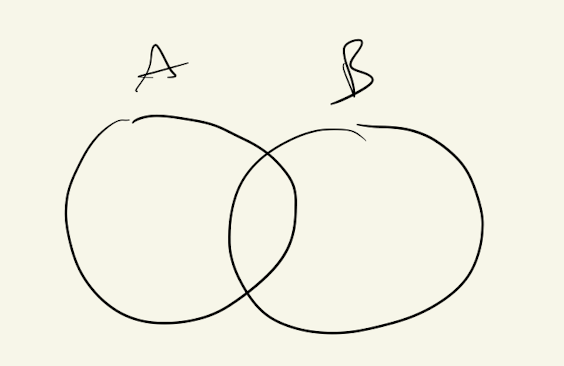
\includegraphics[width=.2\textwidth]{images/two_overlapping_sets}	
 \end{figure}

 \item \label{itm:piece-and-difference} If $A,B \in \F_0$ and $B \subset A$, then   
  \[ \fasf(A) = \fasf(B) + \fasf(A-B)\quad \text{(piece-and-difference decomposition)} \] 
 \begin{figure}[H]
 \centering
 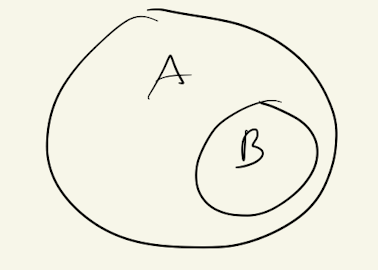
\includegraphics[width=.2\textwidth]{images/whole_and_piece}	
 \end{figure}
 
 \footnote{If the ``piece" satisfies $\fasf(B) < \infty$, we have $\fasf(A-B) = \fasf(A) - \fasf(B) $.  One useful takeaway for piece-and-difference decompositions is that : \textit{the finite measure of the difference is the difference of the finite measures}.}So $\fasf(A) \geq \fasf(B)$ if $\fasf(A-B) \geq 0$. More generally, for non-negative set functions, we have
 \[ \mu_0 (A) \geq \mu_0 (B) \quad \text{(monotonicity)} \] 
 \item \label{itm:subadditivity} Subadditivity holds if $\fasf$ is non-negative, i.e.
 \begin{align*}
 \mu_0 (\cup_{i=1}^n A_i)& \leq \sum_{i=1}^n \mu_0(A_i) \\
  \mu (\cup_{i=1}^\infty A_i)& \leq \sum_{i=1}^\infty \mu(A_i) \\
 \end{align*}
 \end{enumerate}
\label{thm:basic_properties_of_finitely_additive_set_functions}
 \end{theorem}
  
\begin{proof}
 We prove Theorem \ref{thm:basic_properties_of_finitely_additive_set_functions} (b).  The rest is an exercise for the reader (or see the text).
 
 First, we break things into disjoint pieces
 {\footnotesize 
\begin{align*}
A &= \bigg(A \cap B \bigg) \, \bigcupdot \, \bigg(A \cap B^c \bigg)	&& \implies \fasf(A) = \fasf (A \cap B) +  \fasf (A \cap B^c)  && (1) \\
B &= \bigg(A \cap B \bigg) \, \bigcupdot \, \bigg(A^c \cap B \bigg)	&& \implies \fasf(B) = \fasf (A \cap B) +  \fasf (A^c \cap B)  && (2) \\
A \cup B &= \bigg(A \cap B \bigg) \, \bigcupdot \, \bigg(A \cap B^c \bigg) \bigcupdot \, \bigg(A^c \cap B \bigg)	&& \implies \fasf(A \cup B) = \fasf (A \cap B) +  \fasf (A \cap B^c) + \fasf (A^c \cap B)   && (3) 
\end{align*}
}

Summing (1) and (2), we obtain
\[\fasf(A) + \fasf(B) = 2 \fasf(A \cap B) + \fasf(A \cap B^c) + \fasf(A^c \cap B). \]
We use (3) to simplify the RHS, and the result follows.
\end{proof}

\begin{remark}
In the proof of Theorem \ref{thm:basic_properties_of_finitely_additive_set_functions} (b), note that we use a common strategy -- breaking sets into disjoint pieces so that we can apply the assumed (finite or countable) additivity of the set function. 
\end{remark}


\begin{remark}
Is \textit{finiteness} ($|\mu_g (A)| < \infty \; \forall \; A \in \F_g$) equivalent to \textit{boundedness} ($\sup \set{|\mu_g (A)| : A \in \F_g} < \infty$)?
\begin{itemize}
\item $\mu_0, \signedmu$ ? \greencheck
\item $\fasf$ ? \redx (too general)
\end{itemize}
The fact that equivalence holds for signed measures $\signedmu$ is surprising.  Somehow countable additivity compensates for the signedness. See Section 2.1.3 of the text. 
\end{remark}


\subsection{$\S$ 1.2.7-1.2.8: Continuity of countably additive set functions}

Countably additive set functions have a basic continuity property. Continuity of measure is a special case. 

\begin{theorem}
Let $\signedmu$ be a countably additive set function on the \sf\ $\F$. Then

\begin{alphabate}
\item (continuity from below) If $A_1, A_2, ... \in \F$ and $A_n \uparrow A$, then $\signedmu(A_n) \to \signedmu(A)$ as $n \to \infty$.

\begin{figure}[H]
 \centering
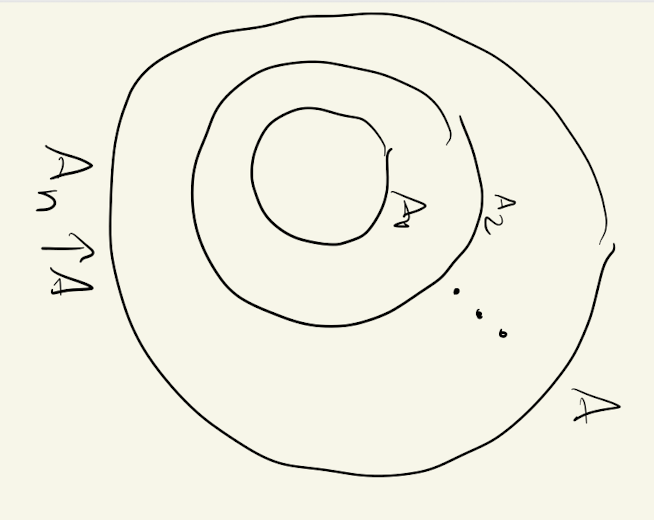
\includegraphics[width=.2\textwidth, angle=90]{images/increasing_sequence_of_sets}	
 \end{figure}
   
\item (continuity from above)  If $A_1, A_2, ... \in \F$, $A_n \downarrow A$, and $\signedmu(A_1)$ is finite, then $\signedmu(A_n) \to \signedmu(A)$ as $n \to \infty$. 
\end{alphabate}
\label{thm:continuity_of_countably_additive_set_functions}
\end{theorem}

\begin{proof}
We prove continuity from below, and leave continuity from above as an exercise to the reader (or see text). 
 
First let us assume that all $\signedmu(A_n)$ are finite (*). Then 
\begin{align*}
A &= A_1 \cupdot (A_2 - A_1) \cupdot (A_3 - A_2) \cupdot ... && 	\text{ by } \eqref{eqn:union_as_disjoint_union_for_increasing_sequences} \\
\implies \signedmu(A) &= \signedmu(A_1) + \signedmu(A_2 - A_1) + \signedmu(A_3 - A_2) + ... && \text{(countable additivity)}\\ 
&= \signedmu(A_1) + \signedmu(A_2) - \signedmu(A_1) + \signedmu(A_3) - \signedmu(A_2) + ... && \text{(Theorem \ref{thm:basic_properties_of_finitely_additive_set_functions} \ref{itm:piece-and-difference}, (*) }\\
&= \ds\lim_{n \to \infty} \signedmu(A_n) && \text{(telescoping difference)}
\end{align*}
Now suppose $\signedmu(A_n) = \infty$ for some $n$.   So write 
\begin{align*}
A &= A_n \cupdot A- A_n && \text{(increasing sequence)}\\ 
\implies \signedmu(A) &= \signedmu(A_n) + \signedmu(A - A_n) && \text{(countable additivity)}\\  
&= \infty + \signedmu(A - A_n) 
\end{align*}

So $\signedmu(A)=\infty$.\footnote{Note that we cannot have $\signedmu(A - A_n)=-\infty$, because that would violate additivity.} Replace $A$ by $A_k$ for any $k \geq n$ to also find $\signedmu(A_k)=\infty$ for all $k \geq n$ and the result follows.

Finally suppose $\signedmu(A_n) = -\infty$ for some $n$. Then the result follows in the same way as for $\signedmu(A_n) = \infty$. 

\end{proof}

\begin{remark}
The logic of the proof of Theorem \ref{thm:continuity_of_countably_additive_set_functions} under the finiteness assumption is as follows.  First, we re-represent the union as a disjoint union (the form is particularly simple since the sets are increasing).  This allows us to apply countable additivity. Then we apply the piece-and-difference decomposition (and the subtraction is defined under the finiteness assumption). 	
\end{remark}



\begin{remark}

In proving Theorem \ref{thm:continuity_of_countably_additive_set_functions}  for the case where $\mu(A_n) = \infty$ for some $n$, it is tempting to make the simpler argument 
\begin{align*}
\mu(A) & \geq \mu(A_n) && \text{(monotonicity)}\\	
\mu(A_k) & \geq \mu(A_n) && \text{(monotonicity)}	 
\end{align*}
for $k \geq n$.  But recall from Theorem \ref{thm:basic_properties_of_finitely_additive_set_functions} that monotonicity only holds under non-negativity, and the theorem statement is more general, applying to \textit{signed} set functions as well. 
\end{remark}

\begin{remark}
Theorem \ref{thm:continuity_of_countably_additive_set_functions} still holds if $\F$ is only assumed to be a field, so long as the limit sets $A$ belong to $\F$.  %We will use this formulation later when we want to extend the set function $\mu(a,b]=b-a$ from a field (of disjoint unions of right semi-closed intervals) to a sigma field. 
\end{remark}

We have the result that finite additivity plus continuity equals countable additivity. 

\begin{theorem}
Let $\fasf$ be a finitely additive set function on the field $\F_0$.  Suppose either
\begin{alphabate}
\item $\fasf$ is continuous from below
\item $\fasf$ is continuous from above at the empty set.	
\end{alphabate}
Then $\fasf$ is countably additive.
\label{thm:finite_additivity_plus_continuity_gives_countable_additivity}
\end{theorem}

\begin{proof}
We prove that the conclusion holds under (a) and leave doing the same for (b) as an exercise to the reader (or see text). 	%To show that $\fasf$ is countably additive, we need to show that  $ \fasf \bigg( \bigcupdot_{n=1}^\infty A_n \bigg) = \ds\sum_{n=1}^\infty \fasf(A_n)$.   

Given $A = \bigcupdot_{n=1}^\infty A_n$, we define $P_n := \bigcup_{m \leq n} A_n$ and so $P_n \uparrow A$.   So we have
\begin{align*}
\fasf(P_n) &\to \fasf(A) && \text{(continuity from below)} \\
\implies \fasf(\bigcup_{m \leq n} A_n) &\to \fasf(A) && \text{(definition)} \\	
\implies \ds\sum_{m=1}^n \fasf(A_n) &\to \fasf(A) && \text{(finite additivity)} \\
\end{align*}
Taking $n \to \infty$ gives countable additivity.
\end{proof}





%By , we have


 %we break up the limit of the increasing sequence into a disjoint union as follows	



 \section{$\S$ 1.3: Extension of measures} \label{sec:extension_of_measures}
 
 
\subsection{Extension and approximation} \label{sec:extension_and_approximation}
 
In Example \ref{ex:lesbesgue_measure}, we discussed the concept of length of a subset of $\R$; in particular, we mentioned extending the set function given on intervals by $\mu(a,b] = b-a$ to a larger class of subsets of $\R$.  


 As remarked in Example \ref{ex:field_of_finite_disjoint_unions_of_rsc_intervals}, if we define $\F_0 = \set{\text{finite disjoint unions of right semi-closed intervals } (a,b], a < b}$, then $\F_0$ is a field, as can be easily verified.  And $\mu$ can easily be seen to be a finitely additive set function on $\F_0$.   

\begin{figure}[H]
\centering
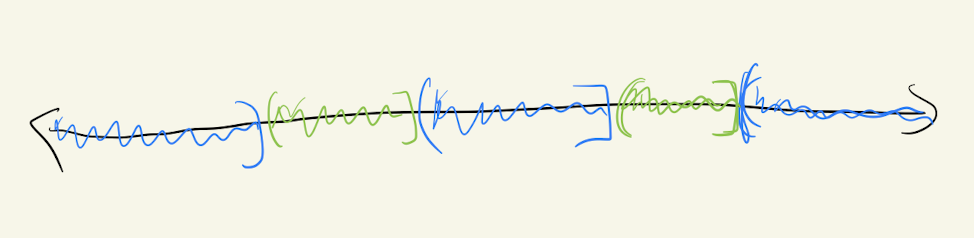
\includegraphics[width=.6\textwidth]{images/rsc_intervals}	
\end{figure}

However, $\F_0$ is not a $\sigma$-field.   So how can we extend this function to a measure on a larger class of subsets?  For instance, we would at least like to be able to measure intervals such as $(a,b), [a,b)$ or $[a,b]$ and points $\set{x}$.   The challenges are:

\begin{itemize}
\item \textit{We need to show that $\mu$ is countably additive.} We will do this in Section 5.   Moreover, in that section, we will generalize our problem to set functions given by $\mu(a,b] = F(b)-F(a)$, where $F$ is an increasing right-continuous function from $\R$ to $\R$.
\item \textit{We need to extend $\mu$ to $\sigma(\F_0)$, the minimal $\sigma$-field containing $\F_0$.} In other words, we need to extend $\mu$ to the Borel sets.  We will handle the problem in this section more generally.  In this section, we will deal with the problem of extending a measure on $\F_0$ to a measure on $\sigma(\F_0)$. We do so using Carath\'eodory's Theorem  (Theorem \ref{thm:caratheodory_extension}).  Along the way, we will use Theorem \ref{thm:extension_of_finite_measure} and Theorem \ref{thm:monotone_class_theorem} to prove Theorem \ref{thm:caratheodory_extension}. 
% We refer to a countably additive set function $\mu$ on a field $\F_0$ as a \textit{pre-measure}
\end{itemize}

 \begin{theorem}
 (Theorem 1.3.6 \cite{ash2000probability}) A finite measure on a field $\F_0$ can be extended to a measure on $\sigma(\F_0)$. 	
 \label{thm:extension_of_finite_measure}
 \end{theorem}

\begin{proof}
See pp. 12-17 of \cite{ash2000probability}.	
\end{proof}

\begin{theorem}{\textbf{(Monotone Class Theorem)}}
Let $\F_0$ be a field of subsets of $\Omega$ and $\C$ be a class of subsets of $\Omega$ that is monotone (if $A_n \in \C$ and $A_n \uparrow 
A$ or $A_n \downarrow A$, then $A \in \C$).  If $\C \supset \F_0$ then $\C \supset \sigma(\F_0)$, then minimal $\sigma$-field over $\F_0$. 
 \label{thm:monotone_class_theorem}
\end{theorem}

\begin{proof}
See pp. 18-19 of \cite{ash2000probability}.	
\end{proof}

\begin{remark}
During the proof of Theorem \ref{thm:monotone_class_theorem}, some key observations are made about the relationship between monotone classes and $\sigma$-fields:
\begin{alphabate}
\item A monotone class that is also field is a sigma-field.  (See Remark \ref{rk:the_limits_of_increasing_and_decreasing_sequences_of_sets_in_a_field_are_also_the_countable_unions}.)
\item The smallest monotone class and smallest sigma-field over a field coincide. 
\end{alphabate}
\label{rk:monotone_classes_and_sigma_fields}
\end{remark}

\begin{remark}{\remarktitle{The utility of the Monotone Class Theorem}}
The Monotone Class Theorem provides an alternate route towards executing on the Good Sets Strategy (Section \ref{sec:good_sets_strategy}.)  Suppose you want to show that all members of a $\sigma$-algebra   $\F$ have some property $P$.  Define ``good sets" as those that satisfy the property
\[ \G := \{ G \in \F : G \text{ has property } P \} \]
The strategy is then to simply
\begin{enumerate}
\item Show $\G$ contains some class $\C$ such that $\F = \sigma(\C)$
\item Show $\G$ is a monotone class.  
\end{enumerate}	 
\label{rk:monotone_class_theorem_for_executing_good_sets_strategy}
\end{remark}

\begin{remark}
The strategy in Remark \ref{rk:monotone_class_theorem_for_executing_good_sets_strategy} is very much like induction.  Step \#1 is the ``base" step and step \#2 is the ``induction" step.
\end{remark}

For an example of where the strategy in Remark \ref{rk:monotone_class_theorem_for_executing_good_sets_strategy} is used, see the proof of uniqueness in the Caratheodory Extension Theorem (Theorem \ref{thm:caratheodory_extension}).  It is also used extensively to show that Borel sets have some property; see Section \ref{sec:properties_of_borel_sets}.


\begin{theorem}{\textbf{(Carath\'eodory Extension Theorem)}} Let $\mu$ be a measure on the field $\F_0$ of subsets of $\Omega$, and assume that $\mu$ is $\sigma$-finite on $\F_0$, so that $\Omega$ can be decomposed as $\cup_{n=1}^\infty A_n$ where $A_n \in \F_0$ and $\mu(A_n) < \infty$ for all $n$.  Then $\mu$ has a unique extension to a measure on $\F := \sigma(\F_0)$, the minimal $\sigma$-field over $\F_0$. 
 \label{thm:caratheodory_extension}
\end{theorem}

\begin{proof} (We follow the argument of \cite{ash2000probability}, but add some detail.) 
First we prove existence.  {\footnotesize [Without loss of generality, we assume the $A_n$ are disjoint.  This is possible because we can use \eqref{eqn:union_as_disjoint_union} to re-express the countable union as a disjoint countable union:  $\Omega = \cup_{i=1}^\infty A_i = \cupdot_{i=1}^\infty B_i$, where $B_i := A_i \cap A_{i-1}^c ... \cap A_1^c$.]  } 

If we define $\mu_n(A)=\mu(A \cap A_n)$ for each $A \in \F_0$, then we can decompose $\mu$ into a countable sum of finite measures:
\begin{itemize}
\item $\mu_n$ is a measure on $\F_0$. {\footnotesize   [Its countable additivity is inherited from $\mu$. If $\cupdot_{i=1}^\infty A_i$ is a disjoint union, then so is $\cupdot_{i=1}^\infty (A_i \cap A_n)$, and $\mu( \cupdot_{i=1}^\infty (A_i \cap A_n)) = \sum_{i=1}^\infty \mu(A_i \cap A_n) $ since $A_i \cap A_n$ are in $\F_0$. ] }
\item $\mu_n$ is finite.  {\footnotesize  [True because $\mu_n(A) = \mu(A \cap A_n) \stackrel{\text{monotonicity}}{\leq} \mu(A_n) < \infty$.]	 }
\item  $\mu = \sum_{n=1}^\infty \mu_n$. {\footnotesize  [True because $\mu(A) = \mu(A \cap \Omega) = \mu(A \cap (\cupdot_{n=1}^\infty A_n)) =\mu(\cupdot_{n=1}^\infty (A \cap A_n)) = \sum_{n=1}^\infty \mu(A \cap A_n) = \mu_n (A). $] }
\end{itemize}
Now by Theorem \ref{thm:extension_of_finite_measure}, we can extend each $\mu_n$ to a measure $\mu_n^*$ on $\F$.   Thus $\mu^* := \sum_{n=1}^\infty \mu_n^*$ extends $\mu$ to $\F$.  Moreover, $\mu^*$ is still a measure since the order of summation in a double series of nonnegative terms can be reversed.  {\footnotesize   [Countable additivity still holds  since:

\begin{align*}
\mu^*(\cupdot_{i=1}^\infty A_i) &= \ds\sum_{n=1}^\infty \mu_n^* (\cupdot_{i=1}^\infty A_i) && \\ &= \ds\sum_{n=1}^\infty \ds\sum_{i=1}^\infty \mu_n^* (A_i) && \tinytext{$\mu_n^*$ is measure, so countably additive}\\
	&= \ds\sum_{i=1}^\infty \ds\sum_{n=1}^\infty \mu_n^*(A_i) && \tinytext{reverse order of summation for double series with non-negative terms} \\
	&= \ds\sum_{i=1}^\infty \mu^*(A_i) && \tinytext{def. of $\mu^*$}
\end{align*}

]. }


Now we prove uniqueness.   That is, we prove that if $\lambda$ is a measure on $\F$ and $\lambda = \mu^*$ on $\F_0$, then $\lambda = \mu^*$ on $\F$.    To see this, as before, we decompose the measure into a sum of finite measures: $\lambda = \sum_{n=1}^\infty \lambda_n$ where $\lambda_n := \lambda (A_n \cap A)$.  Now by assumption $\lambda_n = \mu_n^*$ on $\F_0$.  Where are they equal on $\F$?  Let us define the ``good sets" (recall Section \ref{sec:good_sets_strategy})
\[ \G : = \set{A \in \F : \lambda_n (A) = \mu_n^* (A)} \]
Now we can show $\G = \F$ -- that is, \textit{all} sets in the $\sigma$-field are good sets -- by observing
\begin{itemize} 
\item 	 $\G$ is a monotone class.  {\footnotesize 
[This is true by continuity from below (see Theorem \ref{thm:continuity_of_countably_additive_set_functions}). In particular, a countable union can be considered the limit of an increasing sequence of partial unions (See Remark \ref{rk:the_limits_of_increasing_and_decreasing_sequences_of_sets_in_a_field_are_also_the_countable_unions}.) As a result, the measure of the limiting set is determined, as the limit of the the measure of the sets in that sequence.] }
\item $\G \supset \F_0$. {\footnotesize 
[This is true by construction.] }
\end{itemize} 
And so by Monotone Class Theorem (Theorem \ref{thm:monotone_class_theorem}), we have $\G \supset \F$.  But by construction $\G \subset \F$, and so $\G = \F$.  Therefore $\lambda_n = \mu_n^*$ for each $n$.  

So 
\[ \lambda \stackrel{\text{decomposition}}{=} \sum_n \lambda_n = \sum_n \mu_n^* \stackrel{\text{recomposition}}{=} \mu^*, \] proving uniqueness.
\end{proof}


\begin{remark}
The proof of Theorem \ref{thm:caratheodory_extension} reveals the appeal of $\sigma$-finite measures -- they can be decomposed as the countable sum of finite measures (and the order of summation of double series can be reversed for nonnegative series, so countable additivity still holds). 
\end{remark}


In Remark \ref{rk:monotone_classes_and_sigma_fields} (b), we observed that minimal $\sigma$-fields over a field can be characterized as the minimal monotone classes over a field -- so we merely need to close the field over increasing and decreasing sequences of sets.   This idea suggests that if $\F_0$ is a field and $\F = \sigma(\F_0)$, sets in $\F$ can be approximated in some sense by sets in $\F_0$.  The following result formalizes this notion. 


\begin{theorem}{\textbf{(Approximation Theorem)}} Let $(\Omega, \F, \mu)$ be a measure space.  Let $\F = \sigma(\F_0)$ where $\F_0$ is a field of subsets of $\Omega$.  Let $\mu$ be $\sigma$-finite on $\F_0$.  Then for every $A \in \F$ and fixed $\epsilon >0$, there is a set $B \in \F_0$ such that $\mu( A \triangle B) < \epsilon$.  
\label{thm:approximation theorem}	
\end{theorem}


\begin{example}

This interesting example (from \cite{ash2000probability} pp. 20) provides a counterexample to the theorems when $\F_0$ is not $\sigma$-finite. 

\begin{figure}[h!]
\centering
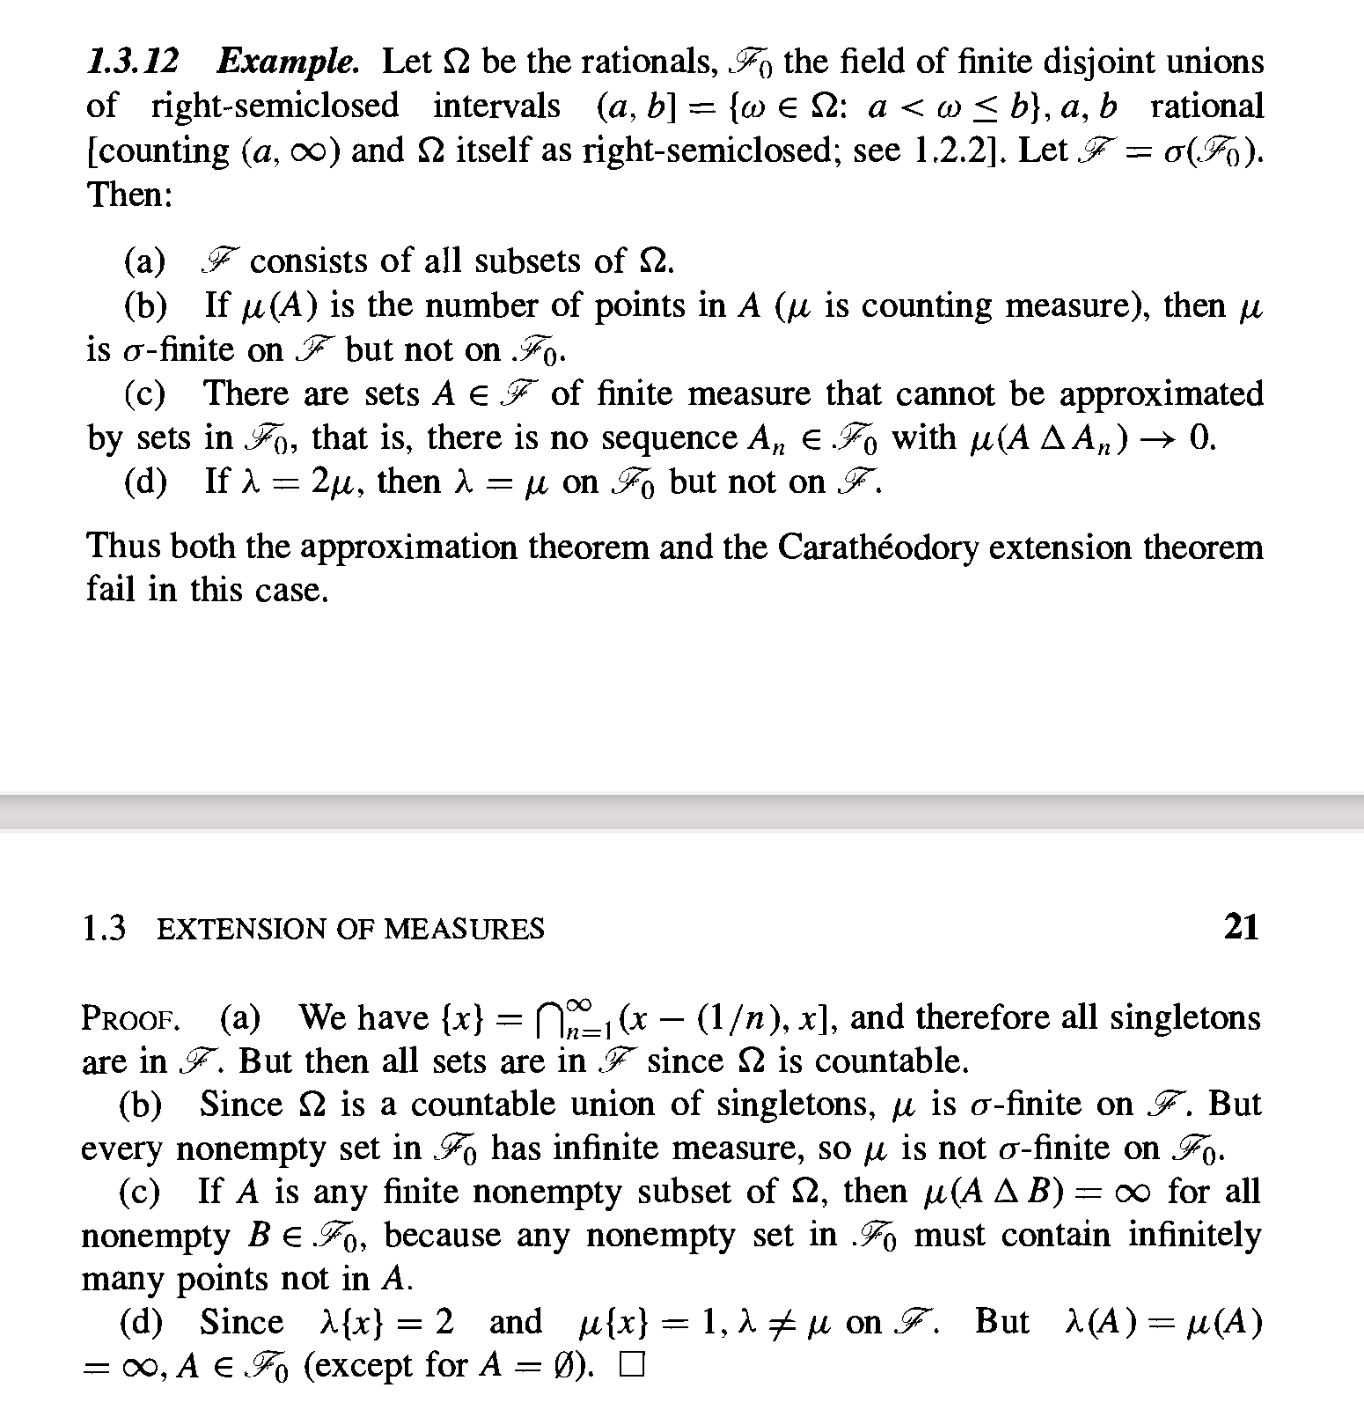
\includegraphics[width=1.\textwidth]{images/example_of_extension}	
\end{figure}
\end{example}

\subsection{Completion of measure spaces}

\begin{definition}
A measure $\mu$ on a $\sigma$-field $\F$ is said to be \textit{complete} iff whenever $A \in F$ and $\mu(A) =0$, we have $B \in F$ for all $B \subset A$.
\end{definition}

\begin{definition}
The \textit{completion} of a measure space $(\Omega, \F, \mu)$ is given by $(\Omega, \F_\mu, \mu)$, where 
\[ \F_\mu := \set{A \cup S : A \in \F, S \subset N 
\text{ for some } N \in \F \text { with } \mu(N) = 0 } \]
and where $\mu$ is extended to $\F_\mu$ by setting $\mu (A \cup S) = \mu(A)$.
\label{def:completion_of_measure_space}
\end{definition}

\begin{remark}
Let us show that Definition \ref{def:completion_of_measure_space} is a valid definition by showing that

\begin{enumerate}
\item \textit{$\F_\mu$ is a $\sigma$-field.}
\item \textit{$\mu$ is a measure on $\F_\mu$.}
\item \textit{The completion is complete.} 	
\end{enumerate}

We justify these in turn:

\begin{enumerate}
\item $\F_\mu$ is closed under countable unions, since 
\[ \cup_{i=1}^\infty (A_i \cup S_i) =  \explaintermbrace{$\in \F$}{(\cup_{i=1}^\infty A_i)} \; \cup \; \explaintermbrace{has measure 0}{(\cup_{i=1}^\infty S_i)} \]
 where the term on the right has measure 0 because $\cup_{i=1}^\infty S_i \subset \cup_{i=1}^\infty N_i \in \F$, and $\mu(\cup_{i=1}^\infty N_i) = \sum_{i=1}^\infty \mu(N_i)= 0$.
 
 $F_\mu$ is also closed under complements, since $S \subset N \implies N^c \subset S^c$, and so
 \[ ( A \cup S)^c = (A^c \cap S^c) = \explaintermbrace{$\in \F$}{(A^c \cap N^c)} \cup \explaintermbrace{has measure 0}{(A^c \cap S^c - N^c)} \]
 where the term on the right has measure 0 by monotonicity, because $A^c \cap S^c - N^c \subset S^c - N^c = S^c \cap (M^c)^c = S^c \cap N \subset N$.
\item First, we show that countable additivity holds in $\F_\mu$. 
\[ \mu(\cupdot_{i=1}^\infty  (A_i \cup S_i)) \stackexplain{see below}{=} \mu(\cupdot_{i=1}^\infty A_i) \stackexplain{$\mu$ countably additive on $\F$ \; }{=} \sum_{i=1}^\infty \mu(A_i) \stackexplain{construction of extension}{=}  \sum_{i=1}^\infty \mu(A_i \cup S_i)  \]
The first equality holds because we can re-represent a disjoint union  $\cupdot_{i=1}^\infty  (A_i \cup S_i) = (\cupdot_{i=1}^\infty A_i) \cup (\cupdot_{i=1}^\infty S_i) $.  Since $\cupdot_{i=1}^\infty S_i  \subset \explaintermbrace{has measure 0 in $\F$}{\cupdot_{i=1}^\infty N_i}$, we have that $\mu((\cupdot_{i=1}^\infty A_i) \cup (\cupdot_{i=1}^\infty S_i)) = \mu(\cupdot_{i=1}^\infty A_i)$. 

Next, we show that $\mu$ is invariant to decompositions: if $A_1 \cup S_1 = A_2 \cup S_2$, then $\mu(A_1 \cup S_1) = \mu(A_2 \cup S_2)$, or more simply $\mu(A_1)=\mu(A_2)$.

\begin{figure}[H]
\centering
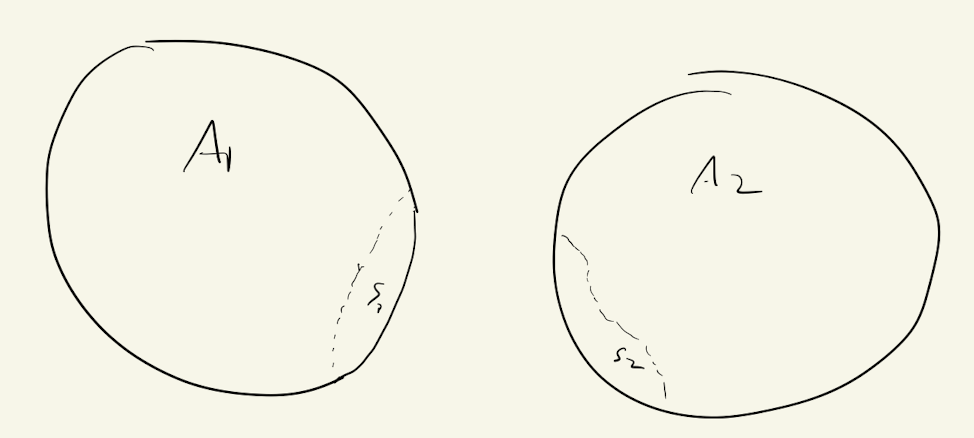
\includegraphics[width=.4\textwidth]{images/completion_of_measure_space}	
\end{figure}

We have    
\[ \mu(A_1)  \stackexplain{countable additivity}{=} \mu(A_1 \cap A_2) + \mu(A_1 \cap A_2^c)\stackexplain{see below}{=} \mu(A_1 \cap A_2) \stackexplain{monotonicity}{\leq} \mu(A_2) \]
where the second equality holds since $A_1 \cap A_2^c \subset S_2$ {\footnotesize (which, in turn, holds since $x \in A_1 \implies x \in A_2 \text{ or } x \in S_2$, so $x \in A_1 \text{ and } x \not\in A_2 \implies x \in S_2$)} .

By symmetry, $\mu(A_2) \leq \mu(A_1)$, so $\mu(A_1)=\mu(A_2)$. 
\item By the definition of a complete measure, we need to show that if $B \in \F_\mu$ and $\mu(B)=0$ then $C \in \F_\mu$ for all $C \subset B$.

%Now $B \in \F_\mu \implies B = \explaintermbrace{$\in \F$}{A} \cup \explaintermbrace{has measure 0}{S}$.  

Now $B \in \F_\mu \implies B = \explaintermbrace{$\in \F$}{A} \cup \explaintermbrace{$\subset N \in \F : \mu(N)=0$}{S}$.  

So our assumption $\mu(B) = 0$ gives us $\mu(A) = 0$, since $\mu(B) = \mu(A \cup S) \stackrel{\text{choice of extension}}{=} \mu(A)  =0$.

Now since we have assumed $C \subset B$ we have
\[\mu(C) \stackexplain{monotonicity}{\leq} \mu(B) \stackrel{B \in \F_\mu}{=} \mu(A \cup S)  \stackexplain{subadditivity}{\leq} \mu(A)+\mu(S)  \stackexplain{see above}{=} 0 + \mu(S) = 0 + 0= 0\]

Since $\mu$ is non-negative, this implies that $\mu(C) =0$.  

We can therefore write $C = \explaintermbrace{$\in \F$}{\emptyset} \cup \explaintermbrace{has measure 0}{C}$, so $C \in \F_\mu$.

Thus, $\mu$ on $\F_\mu$ is complete, since any subset of measure 0 is contained in $\F_\mu$.  
\end{enumerate}
\label{rk:completion_of_measure_space_is_well_defined} 
\end{remark}


 \section{$\S$ 1.4: Lesbesgue-Stieltjes Measures and Distribution Functions} \label{sec:ls_measures_and_distribution_functions}
 
 \begin{definition}
 A \textit{Lesbesgue-Stieltjes measure} on $\R$ is a measure $\mu$ on $\B(\R)$ such that $\mu(I) < \infty$ for each bounded interval $I$.	
 \end{definition}

\begin{definition}
 A \textit{distribution function} on $\R$ is a map $F : \R \to \R$ that is increasing [ $a<b$ implies $F(a) \leq F(b)$] and right continuous [ $\lim_{x \downarrow x_0} F(x) = F(x_0)$]. 
 \end{definition}
 
In this Section, we show that the formula $\mu(a,b] = F(b) - F(a)$ sets up a one-to-one correspondence between distribution functions and Lesbesgue-Stieltjes measures.    

 
 \subsection{$\S$ 1.4.2 Each Lesbesgue-Stietljes measure uniquely determines a distribution function (up to an additive constant)}
 First, the easy part: we show that to every Lesbesgue-Stieltjes  measure, there is a unique distribution function (up to an additive constant). 
 
 \begin{theorem}
 Let $\mu$ be a Lesbesgue-Stietljes measure on $\R$.  Let $\F : \R \to \R$ be defined (up to additive constant) by $F(b)-F(a) = \mu(a,b]$ for $a<b$. Then $F$ is a distribution function.
 \end{theorem}

\begin{proof}
We must show that $F$ is increasing and right continuous.

\begin{enumerate}
\item We have $F(b) - F(a) = \mu(a,b] \geq 0$, since $\mu$ is non-negative. So $F$ is increasing.  
\item By the continuity (from above) of measure (which can be applied since since Lesbesgue-Stietljes measures are finite on any interval), 
\[ \ds\lim_{b' \downarrow b}[F(b') - F(a)] = \ds\lim_{b' \downarrow b} \mu(a,b'] = \mu(a,b]\]

Thus, rearranging,
\[ \ds\lim_{b' \downarrow b} F(b') = \mu(a,b] + F(a) = \bigg(F(b)-F(a)\bigg) + F(a) = F(b)\]
So $F$ is right continuous.  
\end{enumerate}
\end{proof}


  \subsection{$\S$ 1.4.3-1.4.4 Each distribution function (identified up to additive constant) uniquely determines a Lesbesgue-Stietljes measure }
  
 Now the harder part.  We need to show that every distribution function $F$ (identified up to additive constant) uniquely determines a Lesbesgue-Stieltjes  measure.  
 
 We will temporarily work with $\overline{\R}$, because it is a compact space, and then convert back to $\R$.  In $\overline{\R}$, by a similar reasoning as we've seen before (e.g. see Section \ref{sec:extension_and_approximation}), it is straightforward to show that the formula $\mu(a,b] = F(a)-F(b), a,b \in \overline{\R}, a <b$ defines a finitely additive set function on $\F_0(\overline{\R})$, the field of disjoint unions of right semi-closed intervals of the extended reals.  
 
 The challenge will be to show that this set function is countably additive.  If we can do that, then we can apply Carath\'eodory's Extension Theorem to extend the corresponding function $\mu$ on $\F_0(\R)$ to $\B(\R)$, as will be done in Theorem \ref{thm:extension_for_lesbesgue_stietljes_measure}. 

\begin{lemma}
The set function $\mu$ is countably additive on $\F_0(\overline{\R})$.
\label{lemma:ls_measures_are_countably_additive_on_the_field_of_disjoint_rsc_intervals} 	
\end{lemma}

\begin{proof}
We assume $F(\infty) - F(-\infty) < \infty$, so that $\mu$ is finite.   (We leave the case where $F(\infty) - F(-\infty) = \infty$	to the reader, or see the text.)  Our strategy will be to show that $\mu$ is continuous from above, in which case we can apply Theorem \ref{thm:finite_additivity_plus_continuity_gives_countable_additivity} (b) to show that the set function is countably additive.

Let $A_n$ be a sequence of sets in $\F_0(\overline{\R})$ such that $A_n \downarrow \emptyset$.  Now each $A_n$ is a finite union of disjoint r.s.c. intervals.

\begin{figure}[H]
\centering
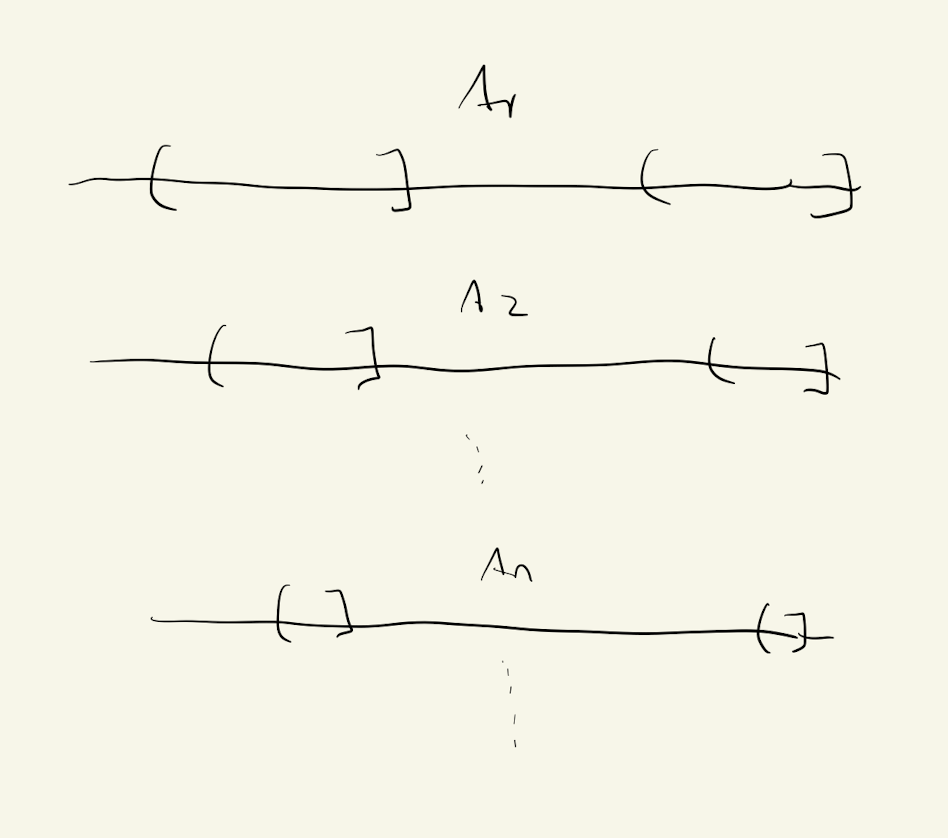
\includegraphics[width=.45\textwidth]{images/decreasing_sequence_of_union_of_rsc_intervals}	
\end{figure}

 Suppose one such interval is $(a,b]$.  By the right continuity of $F$, we can find intervals $(a',b]$ that approximate $(a,b]$ from the inside arbitrarily well, since by continuity from below
\[ \mu(a',b] = F(b) - F(a') \to \mu(a,b] = F(b) - F(a) \text{ as } a' \downarrow a \] 

\begin{figure}[H]
\centering
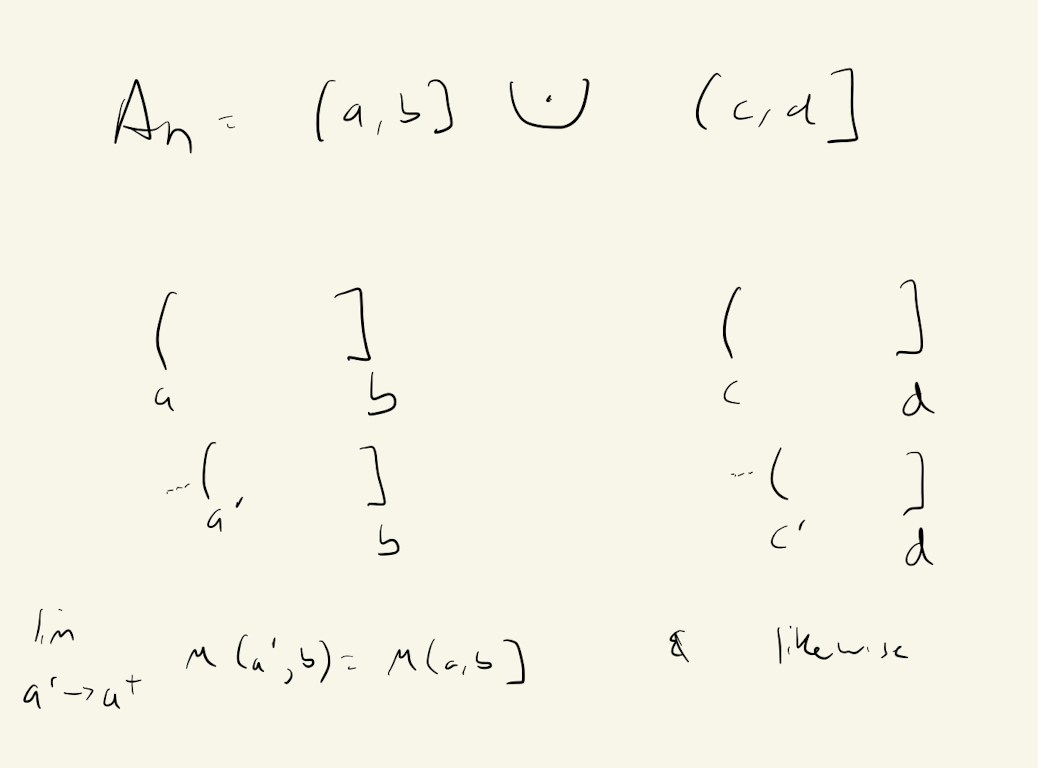
\includegraphics[width=.45\textwidth]{images/approximating_union_of_rsc_intervals}	
\end{figure}

Thus, we can find sets $B_n \in \F_0(\overline{\R})$  where $\mu(B_n)$ approximates $\mu(A_n)$ to any desired $\epsilon > 0$ that satisfy $B_n \subset \overline{B}_n \subset A_n$.  By these inclusion properties and the decreasing nature of the sequence, we have:
\begin{alphabate}
\item $\cap_{n=1}^\infty \overline{B}_n = \emptyset$.	\quad  {[\footnotesize True because each $\overline{B}_n \subset A_n$, so $\cap_{n=1}^\infty \overline{B}_n \subset \cap_{n=1}^\infty A_n = \emptyset$.  ]} 
\item $\cap_{k=1}^n \overline{B}_k = \emptyset$ for sufficiently large $n$.	\quad  {\footnotesize [We have $\overline{\R} \; \stackrel{ \text{item a)}}{=} \; (\overline{\R} - \cap_{n=1}^\infty \overline{B}_n) \; \stackrel{\text{DeMorgan } \eqref{eqn:demorgan_for_relative_complements}}{=} \; \cup_{n=1}^\infty (\overline{\R} - \overline{B}_n)$.   So $\set{\overline{\R} - \overline{B}_n}$ is an open cover of the compact space $\overline{\R}$. By the Heine-Borel theorem, there must be a finite subcover.  So for sufficiently large $n$, we have $\cup_{k=1}^n (\overline{\R} - \overline{B}_k) = \overline{\R}$.  Taking complements of both sides, and once again applying DeMorgan's law \eqref{eqn:demorgan_for_relative_complements} to the relative complement, we find $\cap_{k=1}^n \overline{B}_k = \emptyset$.  ]}
\item $\cap_{k=1}^n B_k = \emptyset$ for sufficiently large $n$. {\footnotesize [This follow from item b) and the fact that each $B_k \subset \overline{B}_k$.]}
\end{alphabate}

So now we use a piece-and-difference decomposition (Theorem \ref{thm:basic_properties_of_finitely_additive_set_functions} (b) ):
\begin{align*}
A_n &= \bigg( \bigcap_{k=1}^n B_k \bigg) \; \bigcupdot \; \bigg(  A_n - \bigcap_{k=1}^n B_k \bigg) && \tinytext{since $\cap_{k=1}^n B_k \subset B_n \subset A_n$} \\
\implies \mu(A_n) &= \mu(\cap_{k=1}^n B_k) \; + \; \mu(A_n - \cap_{k=1}^n B_k) && \tinytext{countable additivity}\\
 &= \cancelto{0}{\mu(\cap_{k=1}^n B_k)} \; + \; \mu(A_n - \cap_{k=1}^n B_k) && \tinytext{for sufficiently large $n$, by item c) above}\\ 
& \leq  \mu( \cup_{k=1}^n (A_k - B_k))&& \tinytext{monotonicity, since $A_n - \cap_{k=1}^n B_k \stackrel{\text{DeMorgan}}{=} \cup_{k=1}^n
(A_n - B_k) \subset \cup_{k=1}^n
(A_k - B_k)$} \\
& \leq \sum_{k=1}^n \mu( A_k - B_k) && \tinytext{finite subadditivity} \\
& = \sum_{k=1}^n \mu( A_k) - \mu(B_k) && \tinytext{piece-and-difference decomposition; also uses finiteness} \\
&\leq \epsilon \sum_{k=1}^n 2^{-k} && \tinytext{Choose $B_k$ such that $\mu(A_k) - \mu(B_k) < \epsilon 2^{-k}$} \\
& < \epsilon. 
\end{align*}

So for sufficiently large $n$, we have $\mu(A_n) < \epsilon$ for any fixed $\epsilon >0$. Thus, $\mu(A_n) \to 0$ for $A_n \downarrow \emptyset$, and so $\mu$ is continuous from above.  So by Theorem \ref{thm:finite_additivity_plus_continuity_gives_countable_additivity} (b), $\mu$ is countably additive.
\end{proof}

\begin{remark}
The proof of Lemma \ref{lemma:ls_measures_are_countably_additive_on_the_field_of_disjoint_rsc_intervals} is a very cool application of Heine-Borel!  In trying to show continuity from above, we started out with an \textit{infinite} intersection of sets.  But in showing continuity, we needed to work with \textit{finite} collection so that we could apply \textit{finite} subadditivity, since that's all we had to use, by assumption. 
\end{remark}

\begin{theorem}
Let $F$ be a distribution function on $\R$, and let $\mu(a,b] = F(b) - F(a), a < b$.  Then there is a unique extension of $\mu$ to a Lesbesgue-Stietljes measure on $\R$.
\label{thm:extension_for_lesbesgue_stietljes_measure}
\end{theorem}

\begin{proof}
See text. 	
\end{proof}

\begin{remark}
The proof of Theorem \ref{thm:extension_for_lesbesgue_stietljes_measure}
essentially directly applies Carathe\'odory's Extension Theorem, since we know from Lemma \ref{lemma:ls_measures_are_countably_additive_on_the_field_of_disjoint_rsc_intervals} that $\mu$ is countably additive on $\F_0(\R)$, a field from which the Borel sets are generated.  The only real additional work is a tedious technical detail to identify a $\mu$-preserving correspondence between sets in $\F_0(\overline{\R})$ (over which we proved countable additivity) and sets in $\F_0(\R)$ (which is the field we actually want to extend).
\end{remark}

  \subsection{$\S$ 1.4.5 Properties of Lesbesgue-Stietljes measures}
 Before extension, we had $\mu(a,b] =F(b) - F(a)$ for $a < b$ where $F$ is a distribution function. The set function $\mu$ was defined only on $\F_0(\R)$, the field of disjoint unions of r.s.c interval.  But after extension, $\mu$ is defined on $\B(\R) = \sigma(\F_0(\R))$, which allows us to measure other types of intervals as well (by expressing those intervals as countable unions or intersections of r.s.c intervals; recall \eqref{eqn:open_intervals_as_rsc_intervals_and_vice_versa}).
 
 \begin{proposition}
 Let $\mu$ be a Lesbesgue-Stieltjes measure, and let $F$ be its associated distribution function.    Let $F(x^-) = \lim_{y \uparrow x} F(y)$. Then 

 \begin{alphabate}
 \item $\mu(a,b] = F(b) - F(a)$	
 \item $\mu(a,b) = F(b^-) - F(a)$	
 \item $\mu[a,b] = F(b) - F(a^-)$	
 \item $\mu[a,b) = F(b^-) - F(a^-)$	
 \item $\mu\set{x} = F(x) - F(x^-)$	
 \item $\mu(-\infty,x] = F(x) - F(-\infty)$	
 \item $\mu(-\infty,x) = F(x^-) - F(-\infty)$	
 \item $\mu(x,\infty) = F(\infty) - F(x)$	
 \item $\mu[x,\infty) = F(\infty) - F(x^-)$	
 \item $\mu(\R) = F(\infty) - F(-\infty)$	
 \end{alphabate}
 \label{prop:properties_of_LS_measures}
\end{proposition}

\begin{proof}
We prove some of these statements and leave the rest to the reader.  

For (b), note that $(a,b) = \cup_{n=1}^\infty (a, b-\frac{1}{n}]$.  So let $A_n = (a, b-\frac{1}{n}]$. Then  by continuity from below,
\[\mu(a,b) = \ds\lim_{n \to \infty}  \mu(A_n) = \ds\lim_{n \to \infty} \big[F(b-\frac{1}{n}) - F(a) \big] = F(b^-) - F (a) \]

For (c), note that $[a,b] = \cap_{n=1}^\infty (a-\frac{1}{n}, b]$.   So by continuity from above (which applies since the sets in the intersection have finite measure),
\[\mu(a,b] = \ds\lim_{n \to \infty} \big[F(b) - F(a - \frac{1}{n}) \big] = F(b) - F (a^-) \]

For (e), note that $\set{x} = \cap_{n=1}^\infty (x-\frac{1}{n}, x]$.   So the statement follows by the same argument as used in (c).

For (i), we can write $[x,\infty) = \cup_{n=1}^\infty [x, x+n)$.  So by continuity from below, 
\[\mu[x,\infty) = \ds\lim_{n \to \infty}  \mu[x, x+n) \stackrel{(d)}{=} \ds\lim_{n \to \infty} \big[ F\big( (x+n)^- \big) - F(x^-) \big] = F(\infty) - F(x^-) \]

For (j), we can write $\R = \cup_{n=1}^\infty [-n, n]$.  So by continuity from below, 
\[\mu(\R) = \ds\lim_{n \to \infty}  \mu[-n,n] \stackrel{(c)}{=} \ds\lim_{n \to \infty} \big[ F(n) - F(-n) \big] = F(\infty) - F(-\infty) \]
\end{proof}


\begin{remark}{\remarktitle{Continuity at a point iffi measure zero at a point}}
\;
\begin{enumerate}
\item Note that
\begin{align*} 
\mu\set{x} = 0 \quad \Leftrightarrow \quad \text{F is continuous at } x
\labelit\label {eqn:continuity_at_a_point_iffi_measure_zero_at_a_point}
\end{align*} 

which holds by Proposition \ref{prop:properties_of_LS_measures} part e) and the fact that $F$ is already right-continuous by definition. 

\item The magnitude of the discontinuity corresponds with the measure of $\set{x}$. 
\end{enumerate}

 For example, the measure corresponding to the distribution function in Figure \ref{fig:distribution_function_with_positive_mass_on_points_that_is_not_concentrated_on_a_countable_set} puts positive probability mass on the points $\set{x_1}, \set{x_2}, \set{x_3}$ and zero probability mass on all other points. 

 \begin{figure}[H]
 \centering
 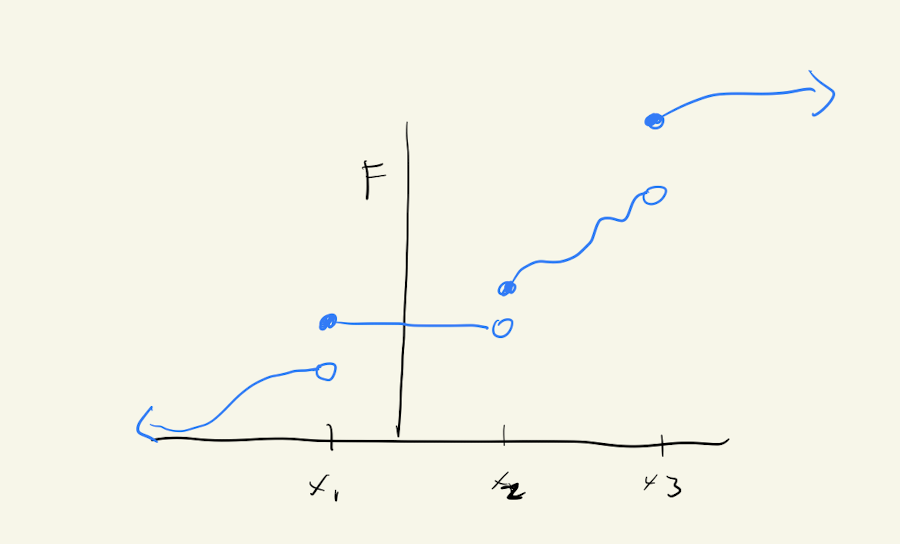
\includegraphics[width=.5\textwidth]{images/distribution_function_with_positive_mass_on_points_that_is_not_concentrated_on_a_countable_set}
 \caption{A distribution function with positive mass on points that is not concentrated on a countable set}	
\label{fig:distribution_function_with_positive_mass_on_points_that_is_not_concentrated_on_a_countable_set}
\end{figure}


%Figure \ref{fig:distribution_function_with_positive_mass_on_points_that_is_not_concentrated_on_a_countable_set} helps to illuminate how working with distribution functions will allow us to cover absolutely continuous, discrete, and mixed random variables in a single paradigm. 
   
\label{rk:continuity_at_a_point_iffi_measure_zero_at_a_point}
\end{remark}

\begin{remark}
The characterization of continuity in Remark \ref{rk:continuity_at_a_point_iffi_measure_zero_at_a_point} in terms of measure zero can be an interesting way to prove continuity, or prove the existence of functions with interesting properties.   For instance, take a countable set $S = \set{x_1, x_2, ...}$ and non-negative weights $\set{w_1, w_2, ...}.$ such that $\sum_i w_i < \infty$.   Then define $\mu(A) = \sum_{i} \set{w_i : x_i \in A}$.  Now $\mu$ is a Lesbesgue-Stietljes measure (and is in fact a finite measure), since $\mu(I) < \infty$ for each bounded interval $I$. By taking $S$ to be the rationals, we have proven the existence of an increasing function $F : \R \to \R$ that is continuous on the irrationals and discontinuous on the rationals {\footnotesize [since each Lesbesgue-Stieltjes measure determines a distribution function $F$ (up to additive constant), and the set of continuities is given by \eqref{eqn:continuity_at_a_point_iffi_measure_zero_at_a_point}]}.
\end{remark}

\begin{remark}{\remarktitle{Lesbesgue-Stieltjes measures of intervals for continuous distribution functions}}
When a distribution function $F$ is continuous rather than simply right continuous, the properties in Proposition \ref{prop:properties_of_LS_measures} reveal that the Lesbesgue-Stieltjes measure of an interval does not depend upon whether the intervals are open or closed, i.e. 
\begin{subequations}
\begin{align}
\mu(a,b] &= \mu(a,b) = \mu[a,b) = \mu[a,b] = F(b)-F(a) &&  \text{for } a \leq b \\
\mu(-\infty,x) &= \mu(-\infty,x] = F(x) - F(-\infty) && \text{for } x \in \R  \\
\mu(x,\infty) &= \mu[x,\infty) = F(\infty) - F(x) && \text{for } x \in \R  
\end{align}
\label{eqn:LS_measures_with_continuous_distribution_function_dont_care_about_intervals_being_open_or_closed}
\end{subequations}

We will informally summarize this as $\mu(a,b]=\mu(a,b)=\mu[a,b)=\mu[a,b]$, where we may take $a,b \in \overline{\R}$ as long as we aren't closing the interval at $\pm \infty$.
\label{rk:LS_measures_with_continuous_distribution_function_agnostic_to_open_vs_closed_intervals}
\end{remark}


\begin{remark}
Note that the properties in Proposition \ref{prop:properties_of_LS_measures} hold even though differences (between a set and a subset) and measures don't commute outside of finite measures.\footnote{See Theorem \ref{thm:basic_properties_of_finitely_additive_set_functions}.}  For instance, if we determine $F$ from the equivalence class by setting $F(-\infty)=0$, then property d) of Proposition \ref{prop:properties_of_LS_measures} says 
\[  \mu[a,b) = \mu(-\infty, b) - \mu(-\infty, a).\]
But we couldn't make that statement by the piece-and-difference decomposition (see Theorem \ref{thm:basic_properties_of_finitely_additive_set_functions}), since $\mu$ isn't necessarily finite.  Thus, continuity of measure lets claim things that the piece-and-difference decomposition does not.
\end{remark}



\subsection{Examples of Lesbesgue-Stieltjes measures on $\R$}

\begin{example}{\remarktitle{Lesbesgue measure}}
Under the identity distribution function ($F(x)=x$), we have $\mu(a,b]=F(b)-F(a)$.  This is known as Lebesgue measure.  Recall from Remark \ref{rk:LS_measures_with_continuous_distribution_function_agnostic_to_open_vs_closed_intervals} that since $F$ is continuous, we also have $\mu(a,b]=\mu(a,b)=\mu[a,b)=\mu[a,b]$.
\label{ex:lesbesgue_measure_as_example_of_lesbesgue_stieltjes} 
\end{example}

\begin{example}{\remarktitle{Generating Lebesgue-Stieltjes measures via integration}}
We can generate a large class of measures on $\B(\R)$ as follows.  Let $f$ be integrable (Reimann for now) on any finite interval, and define
\[ F(b) - F(a) = \ds\int_{a}^b f(t) \, dt\]
which determines $F$ up to an additive constant.   Then $F$ is a distribution function (as it is both increasing and continuous), so it gives rise to a Lesbesgue-Stieltjes measure $\mu(a,b] = F(b) - F(a)$.  Lesbesgue measure (Example \ref{ex:lesbesgue_measure_as_example_of_lesbesgue_stieltjes}) is a special case where $f \equiv 1$.  Once again, Remark \ref{rk:LS_measures_with_continuous_distribution_function_agnostic_to_open_vs_closed_intervals} reveals that by continuity of $F$, we have $\mu(a,b]=\mu(a,b)=\mu[a,b)=\mu[a,b]$.  
\end{example}

\paragraph{A non-example.} All Lesbesgue-Stieltjes measures are sigma-finite. (To see this, simply set $\R = \cup_{n \in \mathbb{N}} (-n,n)$, and observe that $\mu(-n,n)<\infty$.). Here we provide an example of a sigma-finite measure that is not Lesbesgue-Stieltjes.   First, let $\mu$ be concentrated on $S$ (i.e. $\mu(S^c)=0$), where we set $S= \set{1/n : n=1,2,...}$.    Take $\mu\set{1/n}=1/n$ for all $n$.  Since $\R = \cup_{n=1}^\infty {1/n} \cup S^c$, $\mu$ is sigma-finite.  However,
\[  \mu[0,1] \stackrel{\text{countable additivity}}{=} \ds\sum_{n=1}^\infty \df{1}{n} = \infty\]
and so $\mu$ is not a Lesbesgue-Stieltjes measure. 
 
\subsection{Lesbesgue measurable sets}

\begin{definition}
The completion of Lesbesgue measure relative to $\B(\R)$ gives what is known as the \textit{Lesbesgue measurable sets}, denoted $\overline{\B}(\R)$.   
\end{definition}

Each Lesbesgue measurable set is the union of a Borel set and a subset of a Borel set with Lesbesgue measure zero.

\begin{remark}
Sometimes people use the term ``Lesbesgue measure" to refer to

\begin{align*}
\mu : \; & \overline{\B}(\R) \to \R^+
\intertext{as well as}
\mu : \; & \B(\R) \to \R^+
\end{align*}
\end{remark}

\subsection{$\S$ 1.4.6 Lesbesgue-Stieltjes Measures on $\R^n$}

\subsubsection{Overview}
In $\R^n$, as with $\R$, is it possible to establish a one-to-one correspondence between Lebesgue-Stieltjes measures and distribution functions (up to some identification conditions).  However, the details are quite tedious.  

For our purposes, we will focus on
\begin{itemize}
\item Pointing out that, and motivating why, the definition of a distribution function must change in $\R^n$.
\item Showing that if $\mu$ is a \textit{finite} measure on the Borel sets of $\R^n$ and $F(x) = \mu(-\infty, x], x \in \R^n$, then $F$ is a distribution function on $\R^n$ and $\mu(a,b]$ can be provided in terms of it.     (The finite condition can be relaxed, but we omit this here.) %#= \Delta_{(a,b]} F$.
\item Providing some examples of Lesbesgue-Stieltjes distribution functions in $\R^n$. 
%\item Stating the converse -- that if $F$ is a distribution on $\R^n$, there there is a unique Lebesgue-Stieltjes measure associated to it, with $\mu(a,b]$ determined by it. 	
\end{itemize}

 
\subsubsection{Definitions}
The definition of Lesbesgue-Stieltjes measures on $\R^n$ parallels those on $\R$.

\begin{definition}
We define a \textit{right semi-closed interval} (or right semi-closed box) in $\R^n$ as
\[ (a,b] :=	(a_1,b_1] \times ... \times (a_n, b_n]  = \set{x \in \R^n : a_1 < x_1 \leq b_1, ...., a_n < x_n \leq b_n }\]
\end{definition}
\begin{definition}
The \textit{vertices} of a right semi-closed interval in $\R^n$ are given by
\[ V(a,b] = \set{a_1,b_1} \times ... \times \set{a_n, b_n}\]
\label{def:vertices_of_rsc_interval_in_Rn}
\end{definition}

\begin{definition}
The \textit{Borel sets} of 	$\R^n$, denoted $\B(\R^n)$, are those sets which are members of the smallest sigma field containing all right semi-closed intervals $(a,b], a,b \in \R^n$. 
\end{definition}

\begin{definition}
A \textit{Lesbesgue-Stieltjes measure} on $\R^n$ is a measure $\mu$ on $\B(\R^n)$ such that $\mu(I) < \infty$ for each bounded interval $I$. 	
\end{definition}

%We have established how to relate distribution functions and measures when the underlying space is $\R$.  When the underlying space is $\R^n$, the situation is different.

\subsubsection{From (finite) measures on $\B(\R^n)$ to distribution functions}
Recall that in $\R$, we observed the following relation between distribution functions  and Lesbesgue-Stieltjes measures on right semi-closed intervals 
\begin{align*}
\mu(a,b] = F(b) - F(a), \quad a,b \in \R, a<b 
\labelit \label{eqn:measure_as_distribution_function_difference_for_motivating_LS_in_Rn}
\end{align*}
In particular, we observed that given $\mu$, we could construct an $F$ (up to additive constant) via the above relationship.   If we defined $F(-\infty) = 0$, then we could construct $F$ from $\mu$ directly via 
\[ F(x)=\mu(-\infty, x] = \mu(\omega \in \R : \omega \leq x) \]

We would like to to do the same for $\R^n$.  However, note that the equation 
\begin{align*}
\mu(a,b] = F(b) - F(a), \quad a,b \in \R^n, a<b 	
\labelit \label{eqn:measure_as_distribution_function_difference_for_motivating_LS_in_Rn}
\end{align*}
does \textit{not} hold anymore! To see this, let us define  $F : \R^n \to \R$ via 
\[  F(x) = \mu(-\infty, x] = \mu(\omega \in \R^n : \omega_1 \leq x_1, ..., \omega_n \leq x_n)\]

%{\footnotesize We note that that this parallels the situation in $\R$, where  we have $\mu(-\infty, a]=F(a)$ if we identify a member from the equivalence classes of distribution functions by assuming $F(-\infty)=0$.}


\begin{figure}[H]
\centering
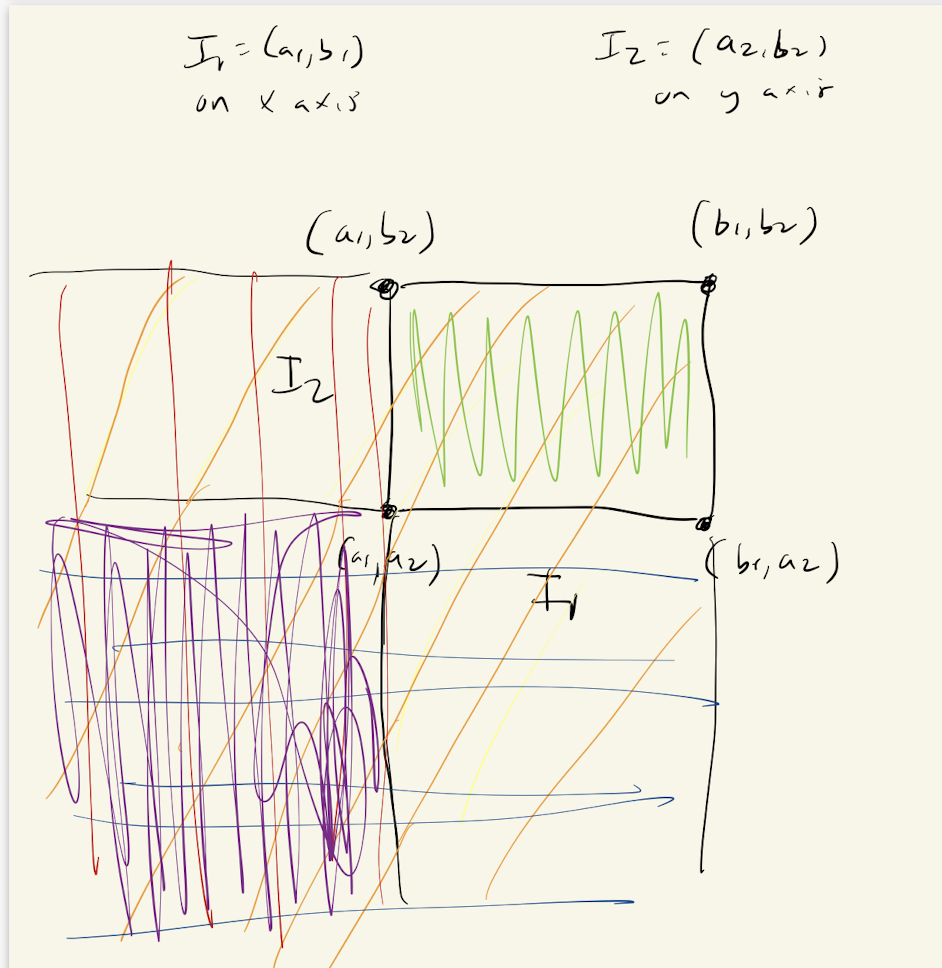
\includegraphics[width=.5\textwidth]{images/distribution_functions_in_Rn}	
\caption{Using a distribution function in $\R^2$ to measure the box $I_1 \times I_2$.}
\label{fig:distribution_functions_in_Rn}
\end{figure}


Now consider Figure \ref{fig:distribution_functions_in_Rn}. We see that if $(a,b] = I_1 \times I_2 = (a_1,b_1] \times (a_2, b_2]$, then 
\begin{align*}
\mu(a,b] &= F(b_1, b_2) - F(a_1, b_2) - F(b_1, a_2) + F(a_1, a_2)
\labelit \label{eqn:measure_of_rsc_interval_in_R2} \\
& \neq F(b_1, b_2) - F(a_1, a_2)
\end{align*}
(Note that we add back in the region that we had double subtracted.)

Now we generalize \eqref{eqn:measure_of_rsc_interval_in_R2} to a formula for measuring r.s.c. intervals in $n$ dimensions, rather than just $2$ dimensions.

\begin{theorem}
Let $\mu$ be a finite measure on $\B(\R^n)$. Define  $F : \R^n \to \R$ via $F(x) = \mu(-\infty, x] = \mu(\omega \in \R^n : \omega_1 \leq x_1, ..., \omega_n \leq x_n)$. Then 
\begin{alphabate}
\item We have 	
	\begin{align*}
	\mu(a,b] &= \Delta_{(a,b]} F  := \Delta_{b_1a_1} \cdots \Delta_{b_na_n} F(x_1, ..., x_n) 
	\labelit \label{eqn:measure_of_rsc_interval_in_Rn_via_distribution_function}
	\intertext{where}
	\Delta_{b_ia_i} G(x_1,...,x_n) &:= G(x_1,....,x_{i-1}, b_i, x_{i+1}, ..., x_n) - G(x_1,....,x_{i-1}, a_i, x_{i+1}, ..., x_n)
	\end{align*}
\item We have
	\begin{align*}
\Delta_{(a,b]} F = \sum_{v \in V(a,b]} (-1)^{\# \text{ of $a_i$'s in v}} \; F(v)
\labelit \label{eqn:computing_area_of_a_rectangle_via_a_distribution}	
	\end{align*}
where $V(a,b]$ are the vertices of $(a,b]$ (see Definition \ref{def:vertices_of_rsc_interval_in_Rn}). 
\end{alphabate}
\label{thm:measure_of_rsc_interval_in_Rn_via_distribution_function}
\end{theorem}

\begin{proof}
We prove part (a) and leave (b) to the reader.
\begin{align*}
\Delta_{b_na_n} &F(x_1, ..., x_n) = 	F(x_1,...,x_{n-1}, b_n) - F(x_1,...,x_{n-1}, a_n)\\
&=\mu(\set{\omega_1 \leq x_1, \; ..., \; \omega_{n-1} \leq x_{n-1}, \; \omega_{n} \leq b_{n}}) - \mu(\set{\omega_1 \leq x_1, \; ..., \; \omega_{n-1} \leq x_{n-1}, \;\omega_{n} \leq a_{n}}) \\
&=\mu(\set{\omega_1 \leq x_1, \; ..., \; \omega_{n-1} \leq x_{n-1}, \; a_n < \omega_{n} \leq b_{n}})
\end{align*}
where the last equality follows by the piece-and-difference decomposition of finite measures.

Similarly, 
\begin{align*}
\Delta_{b_{n-1}a_{n-1}} &\Delta_{b_na_n} F(x_1, ..., x_n) \\
&=\mu(\set{\omega_1 \leq x_1, \;..., \; \omega_{n-2} \leq x_{n-2}, \; a_{n-1} < \omega_{n-1} \leq b_{n-1}, \; a_n < \omega_{n} \leq b_{n}})
\end{align*}
Repeating this, we obtain
\[\Delta_{b_1a_1} \cdots \Delta_{b_na_n} F(x_1, ..., x_n) =  \mu(\set{a_1 < \omega_1 \leq b_1, \; ... \; a_n < \omega_{n} \leq b_{n}}) = \mu(a,b]\]

\end{proof}

\begin{remark}
Note from the proof of Theorem \ref{thm:measure_of_rsc_interval_in_Rn_via_distribution_function} part (a) that the application of the $n$th difference operator restricts the set being measured to the bounds given in the $n$th dimension.  See Figure \ref{fig:applying_the_difference_operator_to_distribution_functions_in_R2}.

\begin{figure}[H]
\centering
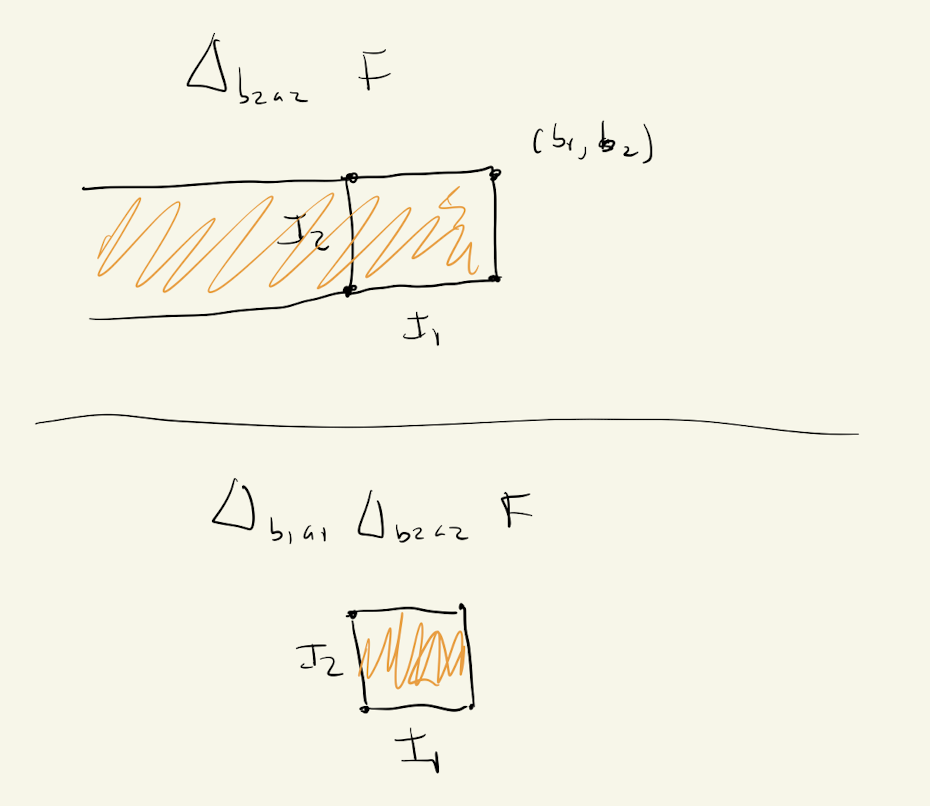
\includegraphics[width=.5\textwidth]{images/applying_the_difference_operator_to_distribution_functions_in_R2}	
\caption{Repeated applications of the difference operator to a distribution function in $\R^2$.}
\label{fig:applying_the_difference_operator_to_distribution_functions_in_R2}
\end{figure}


\end{remark}

\begin{remark}
Equation \eqref{eqn:computing_area_of_a_rectangle_via_a_distribution} tells us that we can measure any $n$-dimensional rectangle in $\R^n$ via $2^n$ evaluations of the distribution function. 
\end{remark}


\subsubsection{Defining distribution functions in $\R^n$}

When defining distribution functions on $\R^n$,  we must alter our notion of \textit{increasing}.     This is due to Theorem \ref{thm:measure_of_rsc_interval_in_Rn_via_distribution_function} part (a).

\begin{definition}
 A \textit{distribution function} on $\R^n$ is a map $F : \R^n \to \R$ that is:
 
 \begin{alphabate}
 \item \textit{increasing}, i.e. its increments must be non-negative in the sense that
 \begin{align*}
 \Delta_{(a,b]} F \geq 0 \quad \text{ for all r.s.c. intervals $(a,b]$}
 \labelit \label{eqn:increasing_condition_for_distribution_functions_on_Rn}
 \end{align*}



 \item \textit{right continuous}, that is
 \[ \ds\lim_{y \downarrow x} F(y) = F(x) \]
 where $y \downarrow x$ means $y_i \downarrow x_i$ for each $i=1,...,n$.
 \end{alphabate}
 \label{def:distribution_function_on_Rn}
 \end{definition}
 
 \begin{remark}
 Note that Definition \ref{def:distribution_function_on_Rn} defines increasing in a different manner than what might be intuitive:
 \[ F(y) \geq F(x) \; \text { if } \; y_i \geq x_i \quad \text{ for all } i=1,...,n\]
 However, such a condition would be insufficient to describe a distribution function in $\R^n.$ For an example of a distribution function that is right continuous and increasing in this sense, but which can assign negative measure to an interval, see pp. 6-7 of \cite{durrett2010probability}.
 \end{remark}

 \subsubsection{From distribution functions on $\R^n$ to Lesbesgue-Stieltjes measures}
 
 \begin{theorem}
 Let $F$ be a distribution function on $\R^n$, and let $\mu(a,b] = F(a,b], a,b \in \R^n, a \leq b$. Then there is a unique extension of $\mu$ to a Lesbesgue-Stieltjes measure on $\R^n$.	
 \end{theorem}
 
 \begin{proof}
 See text. 	
 \end{proof}

\subsubsection{Examples}

Here we provide some examples of how Lesbesgue-Stieltjes measures can be constructed on $\R^n$ via distribution functions.

\begin{enumerate}
\item Let $F_1,F_2,...,F_n$ be distribution functions on $\R$, and define $F(x_1,...,x_n) = F_1(x_1) F_2(x_2) \cdots F_n(x_n)$.  Then $F$ is a distribution function on $\R^n$; it is clearly right-continuous, and it is increasing since
\[ \Delta_{(a,b]} F =\ds\prod_{i=1}^n [F(b_i) - F(a_i)] \geq 0 \]
	
A special case is where each $F_i$ is the distribution function corresponding to Lesbesgue measure on $\B(\R)$.  Then each $F_i(x_i) = x_i$, and so we have
\[ F(x_1,...,x_n) = x_1x_2 \cdots x_n\]
This $\mu$ is \textit{Lesbesgue measure} on $\B(\R^n)$.  Note that 
\[ \mu(a,b] = \Delta_{(a,b]} F = \ds\prod_{i=1}^n (b_i-a_i) \]
and more generally, the Lesbesgue measure of any rectangular box is its volume (which can be seen by using a slight tweak to the arguments of parts (b)-(d) of the proof of Proposition \ref{prop:properties_of_LS_measures}). 
\item Let $f$ be any non-negative function from $\R^n$ to $\R$ such that 
\[ \ds\int_{-\infty}^\infty \cdots  \ds\int_{-\infty}^\infty f(x_1,...,x_n) \; dx_1 \cdots dx_n < \infty \]
(For now, we assume the integration is in the Reimann sense.)

Define 
\[ F(x) = \ds\int_{(-\infty,x]} f(t) dt \]
Then $F$ is a distribution function. It is continuous by the fundamental theorem of calculus, and it is increasing since
\[ \Delta_{(a,b]} F(x) = \ds\int_{a_1}^{b_1} \cdots  \ds\int_{a_n}^{b_n} f(x_1,...,x_n) \; dx_1 \cdots dx_n < \infty \]  
\end{enumerate}

%\begin{exercise}
%We wrote ``more generally, the Lesbesgue measure of any rectangular box is its volume."  Show that, indeed, 
%\[  \mu(a,b]  = \mu(a,b) = \mu[a,b) = \mu[a,b] \]
%for Lesbesgue measure on $\B(\R^n)$.  (Recall that we have shown that these equalities hold for Lesbesgue measure on $\B(\R)$.)
%\end{exercise}

\begin{remark}

It may seem hard to verify \eqref{eqn:increasing_condition_for_distribution_functions_on_Rn}, the condition that a distribution function on $\R^n$ must be increasing.  Not to worry, the recipes above provide straightforward mechanisms for constructing distribution functions on $\R^n$ in which the condition will automatically be verified.
\end{remark}

\subsubsection{Summary}

Let us summarize.\footnote{This passage is basically a paragraph from \cite{ash2000probability} pp. 32 verbatim. However, we alter it slightly here to match our notation.} We have seen that if $F$ is a distribution function on $\R^n$, then there is a unique Lesbesgue-Stieltjes measure determined by $\mu(a,b] = \Delta_{(a,b]} F, a \leq b$.  Also, if $\mu$ is a finite measure on $\B(\R^n)$ and $F(x) = \mu(-\infty, x], x \in \R^n$, then $F$ is a distribution function on $\R^n$ and $\mu(a,b] =  \Delta_{(a,b]} F, a \leq b$.   It is possible to associate a distribution function with arbitrary Lesbesgue-Stieltjes measure on $\R^n$, and thus to establish a one-to-one correspondence between Lesbesgue-Stieltjes measures and distribution fucntions (provided distribution functions with the same increments $\Delta_{(a,b)} F, a,b \in \R^n, a \leq b$ are identified).  However, the result will not be needed, and the details are quite tedious. 

%applying_the_difference_operator_to_distribution_functions_in_R2

% TODO: Define the difference operator, give theorem 1.4.8 but for (b) use the Durrett statement, prove (a) like my notes.  Skip the proof of (b).   Perhaps give the Ash statement for (b) in a remark.  Make a picture and remark for (a) giving the intuition: the $n$th application of the difference operator restricts the set being measured to the bounds given in the $n$th dimension.   Then define distribution functions in R^n.  Finally give the extension statement for $R^n$. 

\subsection{Properties of Borel sets under Lebesgue measure} \label{sec:properties_of_borel_sets}

Below we show some properties of Borel sets that hold under Lesbesgue measure.  How can we accomplish this?  After all, the Borel sets are rather abstractly defined, and although we have been generating them via disjoint unions of r.s.c intervals, they also contain many types of members (e.g., proper open intervals, proper closed intervals, and singletons; bizarre sets like the Cantor set; inverse images of Borel measurable sets under Borel measurable functions; etc.).

To prove that such properties hold, we can take a standard tact: use the the Monotone Class Theorem,  to show that the Borel sets have some property.  Using this approach, we can show that a property holds for \textit{all} Borel sets if we can just show that the property holds for some field generating the Borel sets (e.g., $\F_0 := \set{\text{disjoint unions of } (a,b], a,b \in \R^n }$) -- a much more tangible object to work with.


\begin{remark}{\remarktitle{Using the Monotone Class Theorem to prove that the Borel sets have some property}}
Suppose you want to show that all Borel sets $\B(\R^n)$ have some property $P$.  Define ``good sets" as those that satisfy the property
\[ \G := \{ B \in \B(\R^n) : B \text{ has property } P \} \]
The strategy is then to simply
\begin{enumerate}
\item Show $\G$ contains $\F_0 := \set{\text{disjoint unions of } (a,b], a,b \in \R^n }$.
\item Show $\G$ is a monotone class.  
\end{enumerate}	 
\label{rk:monotone_class_theorem_for_executing_good_sets_strategy_with_borel_sets}
\end{remark}


This is a particular version of the Good Sets Strategy (see Remark \ref{rk:monotone_class_theorem_for_executing_good_sets_strategy}) in the special case where the $\sigma$-field of interest is the Borel sets (and where we take the field generating them to be $\F_0$).  As pointed out in Remark \ref{rk:monotone_class_theorem_for_executing_good_sets_strategy}, this strategy is very much like induction.  Step \#1 is the ``base" step and Step \#2 is the ``induction" step.

For examples where this strategy is used, see the  Approximation Theorem for Borel sets (Theorem \ref{thm:approximation_theorem_for_borel_sets}) or the proof that Lebesgue measure is translation invariant (Proposition \ref{prop:lesbesgue_measure_is_translation_invariant}). We begin with the Approximation Theorem for Borel sets.  This theorem shows that under appropriate conditions, a Borel set can be approximated from below by a compact set, and from above by an open set. 

%\begin{remark}{\remarktitle{Using the Monotone Class Theorem to prove that the Borel sets have some property}} The Borel sets are rather abstract, and also contain many types of members (e.g., proper open intervals, proper closed intervals, singletons, bizarre sets like the Cantor set, etc.).  The MCT gives us a mechanism for showing that some property holds for \textit{all} Borel sets if we can just show that the property holds for some field generating the Borel sets (e.g., $\F_0 := \set{\text{disjoint unions of } (a,b], a,b \in \R^n }$) -- a much more tangible object to work with.  The strategy that is often used is a variant of the Good Sets strategy (see Remark \ref{rk:monotone_class_theorem_for_executing_good_sets_strategy}):  we consider the class of sets that have some desired property, and show that it is a monotone class and contains $\F_0$.  By the Monotone Class Theorem, these two facts are sufficient to prove that some property holds for all Borel sets.  For examples where this is used, see the  Approximation Theorem for Borel sets (Theorem \ref{thm:approximation_theorem_for_borel_sets}) or the proof that Lebesgue measure is translation invariant (Proposition \ref{prop:lesbesgue_measure_is_translation_invariant}).
%\label{rk:utility_of_montone_class_theorem}	
%\end{remark}

%\subsubsection{$\S$ 1.4.11 Approximation theorem for Borel sets}



\begin{theorem}
\textbf{(Approximation Theorem for Borel sets).} If $\mu$ is a $\sigma$-finite measure on $\B(\R^n)$, then for each $B \in \B(\R^n)$,
\begin{alphabate}
\item $\mu(B) = \sup \set{\mu(K) : K \subset B, K \text{ compact}}$
\item If $\mu$ is in fact a Lesbesgue-Stieltjes measure, then
\[ \mu(B) = \inf \set{\mu(V) : V \supset B, V \text{ open}}\]
\item There is an example of a $\sigma$-finite measure on $\B(\R^n)$ that is not a Lebesgue-Stieljes measure for which (b) fails.
\end{alphabate}
\label{thm:approximation_theorem_for_borel_sets}	
\end{theorem}

\begin{proof}
\;
\begin{alphabate}
\item We prove (a) for finite measures.   For the extension to $\sigma$-finite measures, see the text.  

We use the Monotone Class Theorem to show that all Borel sets have the desired property. Let $\G$ be the class of subsets that have the desired property.\footnote{The reader may recognize that we are using the ``good sets" strategy.  See Section \ref{sec:good_sets_strategy} and Remark \ref{rk:utility_of_montone_class_theorem}.} 
	\begin{itemize}
	\item \textit{First, observe that $\G$ contains all compact sets.}  If $K$ is a compact set, then $\mu(K)$ is an upper bound on $\set{\mu(K') : K' \subset K, K' \text{ compact}}$ by monotonicity {\footnotesize [$\mu(K) \geq \mu(K') \text{ for } K' \subset K,  K' \text{ compact}$].}  It is also the least upper bound since for each $\epsilon$, there is a compact $K' \subset K$ satisfying $\mu(K') > \mu(K) - \epsilon$. {\footnotesize [Just take $K'=K$].}  
	\item \textit{Next, we show that $\G$ is a monotone class.}  So we need to show that (i) if $B_n \in \G$ and $B_n \downarrow B$ then $B \in \G$ and (ii) if $B_n \in \G$ and $B_n \uparrow B$ then $B \in \G$.  
		\begin{itemize}
		\item[(i)] Since each $B_n \in \G$, by definition of supremum (see Remark \ref{rk:usage_of_alternate_characterization_of_inf_and_sup}), we can find $K_n \subset B_n$, $K_n$ compact, such that 
		\[\mu(B_n) \leq \mu(K_n) + \epsilon 2^{-n}\]
		Set $K=\cap_{n=1}^\infty K_n$.   Then
		\begin{align*}
		\mu(B) - \mu(K) &= \mu(B-K) && \tinytext{piece-and-difference, $\mu$ finite} \\
		&\stackrel{1}{\leq} \mu(\cup_{n=1}^\infty (B_n-K_n)) && \tinytext{DeMorgan, monotonicity}\\
		&\leq \sum_{n=1}^\infty \mu(B_n - K_n) && \tinytext{countable subadditivity} \\
		&= 	\sum_{n=1}^\infty \mu(B_n) - \mu(K_n) && \tinytext{piece-and-difference, $\mu$ finite} \\
		&= \epsilon 
		\end{align*}
		{\footnotesize [For more detail, Equation (1) applies because $B - \cap_{n=1}^\infty K_n \stackrel{\text{DeMorgan}}{=} \cup_{n=1}^\infty (B-K_n) \stackrel{B \subset B_n}{\subset} \cap_{n=1}^\infty (B_n - K_n)$.]} \\
		
		So for all sets $B$ formed by $B_n \downarrow B$ for $B_n \in \G$, we have that $\mu(B)$ satisfies the second property of the supremum (see Definition \ref{def:supremum_and_infimum}).  {\scriptsize [It satisfies the first property immediately since $K_n \subset B_n  \implies \cap_{n=1}^\infty K_n \subset \cap_{n=1}^\infty  B_n$, so by monotonicity $\mu(K) \leq \mu(B)$, and so $B$ is an upper bound.]} 
		\item[(ii)]  Up to reader or see text for proof. 	
		\end{itemize}
	\item \textit{Now we show that $\G$ contains $\F_0 := \set{\text{disjoint unions of } (a,b], a,b \in \R^n}$}.  Consider that 
	\[ (a,b] = \bigcup_{n=1}^\infty \explaintermbrace{compact}{ \big[a+\frac{1}{n}, b \big] } \]	
	So $[a+1/n, b] \uparrow (a,b]$.  And since $(a,b]$ is the limit of an increasing sequence of compact sets, $(a,b] \in \G$ by the first two bullet points.  A similar argument holds for disjoint unions of sets which have the form $(a,b]$.  
	\item \textit{Now we use the Monotone Class Theorem to finish the proof.} By the previous bulletpoints, $\G$ contains $\F_0 := \set{\text{disjoint unions of } (a,b], a,b \in \R^n}$, and $\G$ is a monotone class.  So by the Monotone Class Theorem (Theorem \ref{thm:monotone_class_theorem}), $\G$ contains $\sigma(\F_0) = \B(\R^n)$.\footnote{In other words, \textit{all} Borel sets are are ``good" - they have the property stated in part (a).}  
	\end{itemize}


\item We prove part (b) for finite measures.  For the extension to $\sigma$-finite measures, see the text.

We have 
\begin{align*}
\mu(B) & \stackrel{1}{\leq}	\inf \set{\mu(V) : V \supset B, V \text{ open}} && \tinytext{by monotonicity and Definition \ref{def:supremum_and_infimum}} \\
 & \stackrel{2}{\leq}	\inf \set{\mu(K^c) : K^c \supset B, K \text{ compact}} && \tinytext{by monotonicity and Proposition \ref{prop:sup_and_inf_for_subsets_are_tighter}} \\
 &= \inf \set{\mu(\R^n) - \mu(K) : K \subset B^c, K \text{ compact}} && \tinytext{by piece-and-difference, $\mu$ finite} \\
 & \stackrel{3}{=}	\mu(\R^n) - \sup \set{\mu(K) : K \subset B^c, K \text{ compact}} && \tinytext{by Proposition \ref{prop:sup_and_inf_for_minkowski_sum_and_diff}} \\
  & =	\mu(\R^n) - \mu(B^c)  && \tinytext{by part (a)}\\
&= \mu(B)
\end{align*}
For more details, Equation (1) holds since, by monotonicity, the LHS is a lower bound on the RHS, so the statement must be true by definition of infimum. Equation (2) holds since the LHS is a smaller set than the RHS (because not every open set is the complement of a compact set)\footnote{Recall that in $\R^n$, a compact set is both closed \textit{and} bounded.}, and the infimum can only increase on subsets by Proposition \ref{prop:sup_and_inf_for_subsets_are_tighter}. Equation (3) holds by writing $\mu(K^c) = \mu(\R^n) - \mu(K)$.  This has the form of a Minkowski set difference $A = \set{c} - B$, where $c$ is a singleton.  So we have $\inf A = \inf ( \set{c} - B) \stackrel{Prop. \ref{prop:sup_and_inf_for_minkowski_sum_and_diff}}{=} \inf \set{c} - \sup B = c - \sup B$. 
\item See the text.
\end{alphabate}
 
 \end{proof}

%\subsubsection{Translation Invariance of Lebesgue Measure}

\begin{proposition}
\textbf{(Translation Invariance of Lebesgue Measure).} Lebesgue measure is translation invariant.  That is, if $B \in \overline{\B}(\R^n)$ and $c \in \R^n$, then $B+c \in  \overline{\B}(\R^n)$ and $\mu(B+c)=\mu(B)$, where $\mu$ is Lesbesgue measure.	
\label{prop:lesbesgue_measure_is_translation_invariant}
\end{proposition}

\begin{proof}
We prove the statement for $\B(\R^n)$ and leave the extension to $\overline{\B}(\R^n)$ to the reader. We shall use the Monotone Class Theorem as our vehicle for executing the Good Sets Strategy (see Remark \ref{rk:monotone_class_theorem_for_executing_good_sets_strategy}).  That is, we will let $\G$ be the class of ``good sets" that have the desired property. Then we must show: (a) that $\G$ is a monotone class and (b) that $\G$ contains $\F_0 = \set{\text{disjoint union of sets of the form } (a,b], a, b \in \R^n}$. We will use this strategy twice, to show: (1) that $B \in \B(\R^n)$ and $c \in \R^n$ implies $B+c \in  \B(\R^n)$  (2) that $\mu(B+c)=\mu(B)$ for all $B \in \B(\R^n)$.  

\begin{enumerate}
\item We want to show that $B \in \B(\R^n) \implies B+c \in \B(R^n)$.  Let $\G$ be the sets where the property holds.
	\begin{alphabate}
	\item Consider a sequence $B_n \uparrow B$ such that $B_n \in \G$.  That is, by hypothesis, we have $B_n \in \B(\R^n) \implies B_n+c \in \B(R^n)$.  Then 
	\[  B+c = (\bigcup_{n=1}^\infty B_n) + c = \bigcup_{n=1}^\infty \explaintermbrace{\quad in $ \B(\R^n)$ \, by hypothesis}{(B_n + c)} \explaintermbrace{\quad by $\sigma$-field}{\in \B(\R^n)}\]
	So $B \in \G$.
	\item This property holds on $\F_0$; that is $\G \supset \F_0$.   Given $(a,b] \in \F_0, (a,b]+c = (a+c,b+c] \in \F_0$.  A similar statement holds for disjoint unions of r.s.c. intervals. 
	\end{alphabate}
\item We want to show that $\mu(B+c)=\mu(B)$ for all $B \in \B(\R^n)$.
	\begin{alphabate}
	\item Let $\G$ be the sets where the property holds. We show $\G$ is a monotone class. \\
	 
	 First, we handle increasing sequences. So we want to show $B_n \in \G, B_n \uparrow B \implies B \in G$.   Now by hypothesis, $\mu(B_n + c) = \mu(B_n)$.  So 
	 \begin{align*}
	 \mu(B+c) &=  \mu \big( \cup_{n=1}^\infty (B_n)+c \big)  && \tinytext{def. of $B$} \\
	  &=  \mu \big( \cup_{n=1}^\infty (B_n+c) \big)  && \tinytext{def. of union and +; still an increasing sequence} \\
	 &= \ds\lim_{n \to \infty} \mu(B_n+c)  && \tinytext{continuity from below} \\
	 &= \ds\lim_{n \to \infty} \mu(B_n) && \tinytext{hypothesis} \\
	 &= \mu(B) && \tinytext{continuity from below}
	 \end{align*}
 
 	Now we handle decreasing sequences.  So we want to show $B_n \in \G, B_n \downarrow B \implies B \in G$.  We could use the same argument as above with continuity from above instead of continuity from below, but continuity from above only applies for sets with finite measure.  However, Lesbesgue measure is $\sigma$-finite, so we can handle this problem in the standard way.\footnote{In particular, we write $\Omega = \cupdot_{n=1}^\infty \Omega_n$ where $\mu (\Omega_n) < \infty$.\footnote{Recall that we can represent any union as a disjoint union; see Section \ref{sec:representing_unions_as_disjoint_unions}.}  Then we define a finite measure $\mu_n$ via $\mu_n(A) := \mu(A \cap \Omega_n)$.  We have 
 		\[ \mu(A) = \sum_{n=1}^\infty \mu_n(A), \quad (*)\]
 		since $\mu(A) = \mu(\cupdot A \cap \Omega_n) = \sum_n \mu(A \cap \Omega_n) = \sum_n \mu_n(A)$.
 		
 		Now, using the continuity from above argument for finite measures, we have 
 			\[ \mu_n(B+c) = \mu_n(B), \quad (+)\]
 			
 		And so
 		\[\mu(B+c) \stackrel{(*)}{=} \sum_n \mu_n (B+c)   \stackrel{(+)}{=}  \sum_n \mu_n(B) \stackrel{(*)}{=} \mu(B)  \]
 	}
% 	 \begin{align*}
%	 \mu(B+c) &\leq \mu(B) + \mu(c) && \tinytext{countable subadditivity} \\
%	 &= \ds\lim_{n \to \infty} [\mu(B_n)] + \mu(c) && \tinytext{continuity from below} \\
%	 &= \ds\lim_{n \to \infty} [\mu(B_n) + \mu(c)] && \tinytext{limit properties} \\
%	 &= \ds\lim_{n \to \infty} [\mu(B_n)] && \tinytext{hypothesis} \\
%	 &= \mu(B) && \tinytext{continuity from below}
%	 \end{align*}
% 
% 	\red{I AM ON DRUGS, THIS DOESNT HOLD}
	\item Now we show that $\G$ contains $\F_0$. The property certainly holds for r.s.c intervals; that is, $\mu(a+c,b+c] = \mu(a,b]$. \footnote{ For example, in $\R$, we have
	\[ \mu\big( (a,b] + c \big) = \mu\big( (a+c,b+c]\big) =(b+c) - (a+c) = b-a = \mu(a,b]\] 
	}  For Lesbesgue measure on $\R^n$, the distribution function is $F(x_1, ..., x_n) = x_1 \cdots x_n$, and so $\mu (a,b] = \Delta_{b_1 a_1} \cdots \Delta_{b_n a_n} [x_1 \cdots x_n]$. Now note that
		\begin{align*}
		\Delta_{b_i + c_i, a_i+c_i} [x_1 \cdots x_n] &= x_1 \cdots x_{i-1} \bigg( (b_i + c_i) - (a_i + c_i)  \bigg) x_{i+1} \cdots x_n \\
		& = x_1 \cdots x_{i-1} \bigg( b_i - a_i  \bigg) x_{i+1} \cdots x_n \\
		&= \Delta_{b_i a_i} [x_1 \cdots x_n]  
		\end{align*}
	So $\Delta_{b_i + c_i, a_i+c_i} = \Delta_{b_i, a_i}$ for each $i=1,..n$.  Thus,  
	\[ \mu(a+c,b+c] = \Delta_{b_1+c_1, a_1 +c_1} \cdots \Delta_{b_n+c_n, a_n+c_n} [x_1 \cdots x_n] = \Delta_{b_1 a_1} \cdots \Delta_{b_n a_n} [x_1 \cdots x_n] = \mu(a,b] \] 
	A similar proof holds for disjoint unions of r.s.c intervals.
	\end{alphabate}
\end{enumerate}

\end{proof}

\subsection{A set that is not Lesbesgue measurable} \label{sec:set_that_is_not_lesbesgue_measurable}

\begin{proposition}
Call $x,y \in \R$ equivalent iff $x-y \in \mathbb{Q}$.\footnote{So, for example, some equivalence classes are:
\begin{itemize}
\item $e \sim e + \frac{1}{10} \sim e - \frac{1}{10} \sim e+\frac{50}{3} \sim ...$
\item  $\pi \sim \pi + \frac{1}{10} \sim \pi - \frac{1}{10} \sim \pi+\frac{50}{3} \sim ...$
\item $1 \sim 1 + \frac{1}{10} \sim 1 - \frac{1}{10} \sim 1 +\frac{50}{3} \sim ...$
\end{itemize}
} Define $A \subset [0,1]$ as a set containing one member from each class. (This set exists by axiom of choice.) Then $A$ is not Lesbesgue measurable.

\label{prop:existence_of_set_that_is_not_lesbesgue_measurable}
\end{proposition}

\begin{proof}
\begin{alphabate}
\item First, we show that we can partition the reals as $\R = \bigcupdot_{q \in \mathbb{Q}} (q+A)$.  
	\begin{itemize}
		\item \textit{(disjointedness)} Suppose $x \in q+A$ and $x \in r+A$ for some $r,q \in \mathbb{Q}, r \neq q$.  Then $\exists\, a_1,a_2 \in A : q + a_1 = r + a_2 \implies a_1 - a_2 = r - q$.   Now since $r \neq q$, we know that $a_1$ and $a_2$ are not the same.  But they are in the same equivalence class, since $r-q \in \mathbb{Q}$. This  contradicts how $A$ was constructed.
		\item \textit{(containment)} We show $\R \subset \bigcupdot_{q \in \mathbb{Q}} (q+A)$ (as the other direction is obvious).  If $x \in \R$ and $a_x$ is its representative in $A$, then $x-a_x = q \in \mathbb{Q}$, and so $x \in q + A$. %x is in A translated by q.
	\end{itemize}
\item Now we note that since $A \subset [0,1]$, we have 
\[ \bigcupdot_{q \in \mathbb{Q}, 0 \leq q \leq 1} (q + A) \subset [0,2] \]
So 
\[ 2 = [0,2] \stackreltext{subadditivity}{\geq} \mu\bigg(\bigcupdot_{q \in \mathbb{Q}, 0 \leq q \leq 1} q + A \bigg)  = \ds\sum_{q \in \mathbb{Q}, 0 \leq q \leq 1} \mu(q+A) \stackreltext{translation invariance}{=} \ds\sum_{q \in \mathbb{Q}, 0 \leq q \leq 1}  \mu(A) \]
This implies $\mu(A) = 0$, since the RHS of this equation is a countable sum of a constant, and so can only take on values $0$ or $\infty$.
	
But then 
\[ \infty = \mu(\R) \stackreltext{part (a)}= \mu \bigg(\bigcupdot_{q \in \mathbb{Q}} (q+A) \bigg)
= \ds\sum_{q \in \mathbb{Q}} \mu(q+A) 
 \stackreltext{translation invariance}{=}   \ds\sum_{q \in \mathbb{Q}} \mu(A) \stackreltext{see above}{=} 0. \;    \contradiction \]

\end{alphabate}

	
\end{proof}

\begin{remark}
The proof of Proposition \ref{prop:existence_of_set_that_is_not_lesbesgue_measurable} only used the following two properties of Lesbesgue measure:
\begin{itemize}
\item translation invariance
\item finiteness on bounded intervals %(note that the argument in part (b) would go through for any bounded interval $[a,b]$ by the choice of bounds on $A$ and on the rationals used in part (b)). % Commented this out because it's outdated and possibly no longer relevant
\end{itemize}
Therefore, our argument shows that there cannot be a translation invariant measure $\lambda$ (except $\lambda \equiv 0$) on the class of all subsets of $\R$ such that $\lambda(I) < \infty$ for all bounded intervals $I$.
\label{rk:implications_of_existence_of_set_that_is_not_lesbesgue_measurable}
\end{remark}

% Commented the question out because it's outdated and possibly no longer relevant
%\begin{question}
%Our discussion in Remark \ref{rk:implications_of_existence_of_set_that_is_not_lesbesgue_measurable} parallels that of \cite{ash2000probability} pp. 35.  But haven't we actually proved a stronger result - namely that there cannot be a translation invariant measure $\lambda$ (except $\lambda \equiv 0$) on the class of all subsets of $\R$ such that $\lambda(I) < \infty$ for \textit{any} bounded interval $I$?
%\end{question}

\section{$\S$ 1.5 Measurable functions and Integration}

In this section, we will introduce the general theory of integration of a function with respect to a general measure, as introduced by Lebesgue.  We will sometimes refer to this as \textit{Lesbesgue integration}.  However, that term is sometimes used to refer to the special case of integration of a function defined on a sub-domain of the real line with respect to the Lebesgue measure. To be more precise, some authors (e.g. \cite{ash2000probability}) refer to the former as \textit{abstract Lesbesgue integration}.  We will differentiate between the general and special cases by referring to \textit{Lesbesgue integration} (which can be against arbitrary measure) and \textit{Lesbesgue integration against Lesbesgue measure}.

\subsection{Intuition\footnote{Here we borrow freely from some sections of Wikipedia.}} \label{sec:intuition_on_lesbesgue_integration}

Folland summarizes the difference between the Riemann and Lebesgue approaches thus: ``to compute the Riemann integral of $f$, one partitions the domain [...] into subintervals", while in the Lebesgue integral, ``one is in effect partitioning the range of $f$ " \cite{folland1999real}.

\begin{figure}[H]
\centering 
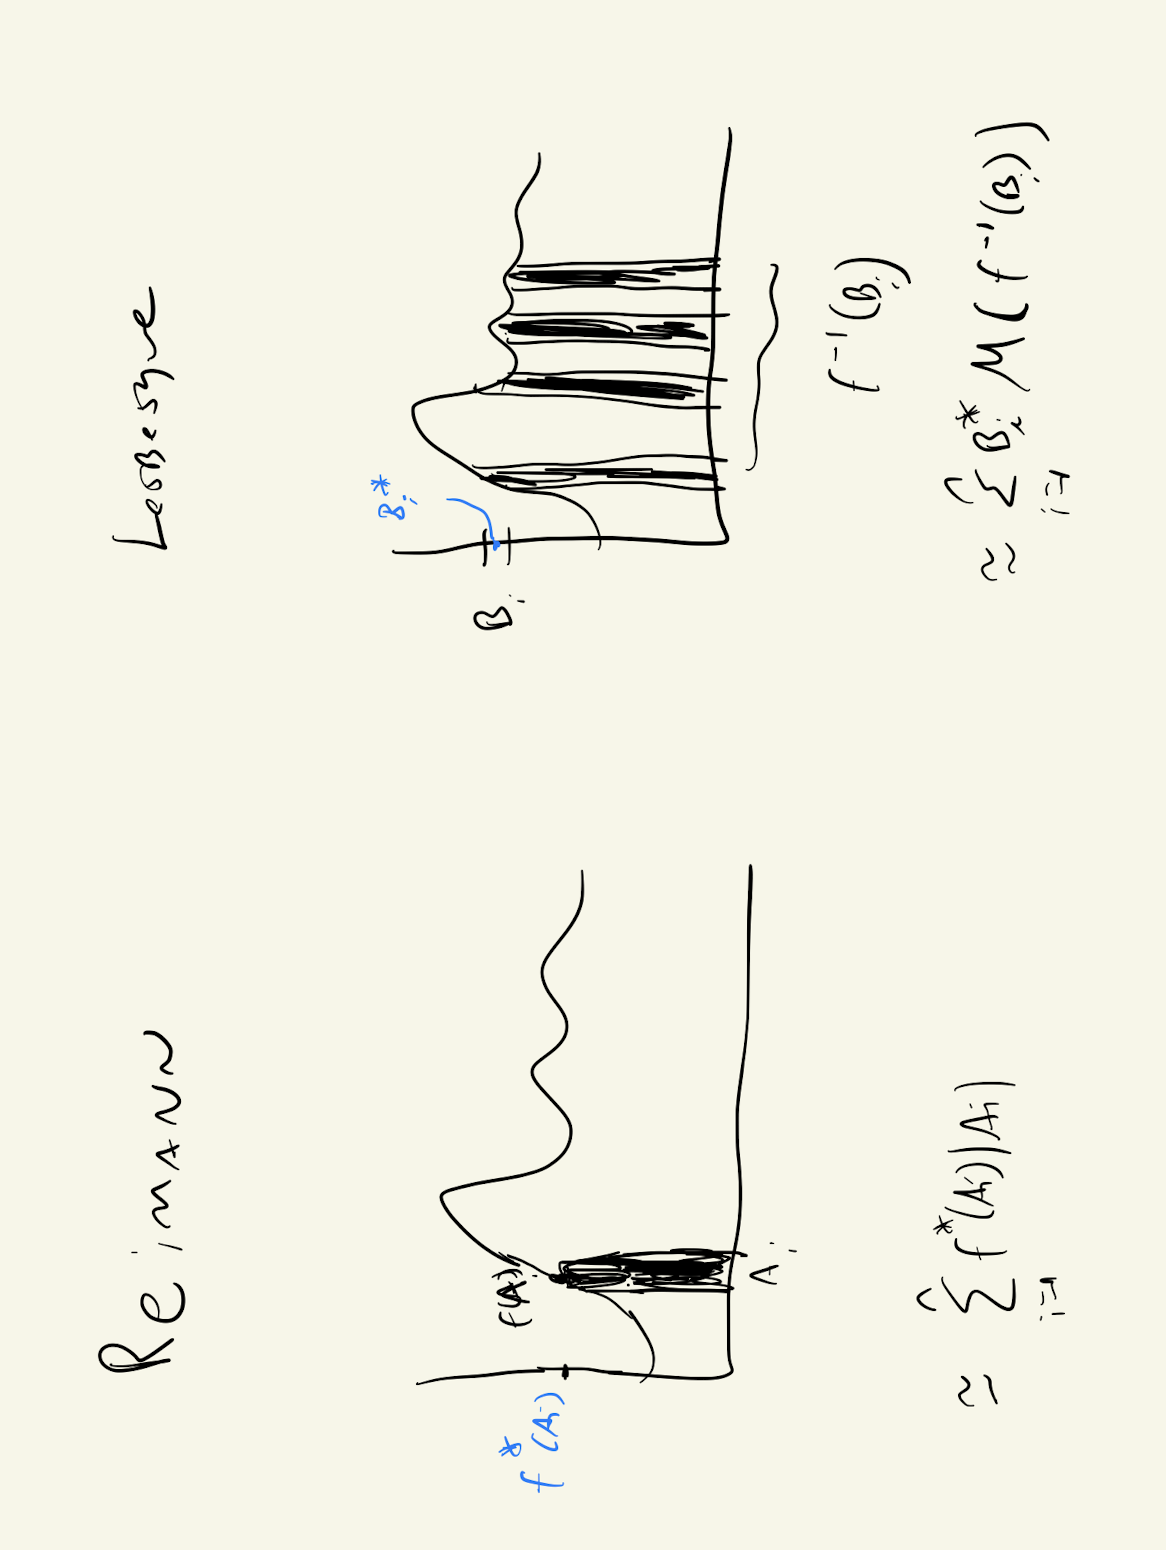
\includegraphics[width=.7\textwidth, angle=270]{images/lesbesgue_vs_reimann}
\end{figure}


Similarly, suppose we want to find a mountain's volume (above sea level).

\begin{itemize}
\item \textbf{The Riemann approach}: Divide the base of the mountain into a grid of 1 meter squares. Measure the altitude of the mountain at the center of each square. The volume on a single grid square is approximately 1 $m^2$ × (that square's altitude), so the total volume is 1 $m^2$ times the sum of the altitudes.
\item \textbf{The Lebesgue approach}: Draw a contour map of the mountain, where adjacent contours are 1 meter of altitude apart. The volume of earth a single contour contains is approximately 1 m × (that contour's area), so the total volume is the sum of these areas times 1 m.

\begin{figure}[H]
\centering 
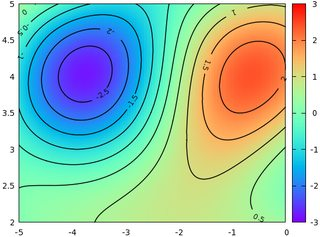
\includegraphics[width=.5\textwidth]{images/contour_plot}
\end{figure}
\end{itemize}

While the Riemann integral considers the area under a curve as made out of vertical rectangles, the Lebesgue definition considers horizontal slabs that are not necessarily just rectangles, and so it is more flexible. For this reason, the Lebesgue definition makes it possible to calculate integrals for a broader class of functions. For example, as we will see, the \textit{Dirichlet function}, which is 0 where its argument is irrational and 1 otherwise, has a Lebesgue integral, but does not have a Riemann integral.



Lebesgue summarized his approach to integration in a letter to Paul Montel:
\begin{quotation}
I have to pay a certain sum, which I have collected in my pocket.  I take the bills and coins out of my pocket and give them to the creditor in the order I find them until I have reached the total sum. This is the Riemann integral. But I can proceed differently. After I have taken all the money out of my pocket I order the bills and coins according to identical values and then I pay the several heaps one after the other to the creditor. This is my integral.
\end{quotation}



The insight is that one should be able to rearrange the values of a function freely, while preserving the value of the integral.  This process of rearrangement can convert a very pathological function into one that is ``nice" from the point of view of integration, and thus let such pathological functions be integrated.


\subsection{$\S$ 1.5.1 Measurable functions}

\subsubsection{Definitions}

\begin{definition}
If $\F$ is a $\sigma$-field of subsets of $\Omega$, then $(\Omega, \F)$ is called a \textit{measurable space} and sets in $\F$ are called \textit{measurable sets}.
\label{def:measurable_space_and_measurable_sets}	
\end{definition}

We can now define measurable functions as those which preserve measurability under inverse images.
   
\begin{definition}
If $h : \Omega_1 \to \Omega_2$, $h$ is a \textit{measurable function} relative to the $\sigma$-fields $\F_j$ of subsets of $\Omega_j$, $j=1,2$, iff $h^{-1}(A) \in F_1$ for all $A \in \F_2$.  We sometimes denote measurable functions as an explicit mapping between measurable spaces: $h : (\Omega_1, \F_1) \to (\Omega_2, \F_2)$.
\label{def:measurable_function}
\end{definition}


Borel measurable functions are a special case of particular interest.  
 
\begin{definition}
A \textit{Borel measurable function} is a measurable function $h : (\Omega_1, \F_1) \to (\R^n, \B(\R^n))$ or  $h : (\Omega_1, \F_1) \to (\overline{\R}^n, \B(\overline{\R}^n))$.  
\label{def:borel_measurable_function}
\end{definition}

Note that the \textit{Borel} in Borel measurability refers to the measurable sets in the \textit{range}, not the domain.  However, when applying Definition \ref{def:borel_measurable_function}, if $\Omega_1$ is a Borel subset of $\R^k$ or $\overline{\R}^k$, we assume $\F_1 = \B$.

\subsubsection{``Computational" definitions}
In practice, to show that a function is measurable, it suffices to apply what we might call the ``computational definition of measurable functions."

\begin{claim}{\remarktitle{Computational definition of measurable functions}}
For $h : \Omega_1 \to \Omega_2$ to be measurable relative to the $\sigma$-fields $\F_j$ of subsets of $\Omega_j$, $j=1,2$, it suffices to show that $h^{-1}(B) \in \F_1$ for all $B \in \C : \sigma(\C) = \F_2$. 
\label{claim:computational_def_measurability}	
\end{claim}

\begin{proof}
We apply the ``Good Sets" strategy (see Section \ref{sec:good_sets_strategy}).  The ``base" condition is satisfied by hypothesis.  For the ``induction step", we need to show that the good sets form a $\sigma$-field.

Let us define the good sets as $\G := \set{B \in \F_2 : h^{-1}(B) \in \F_1}$.  We check the three conditions:
\begin{itemize}
\item $\Omega_2 \in \G$	? \greencheck.  True because $h^{-1}(\Omega_2) = \Omega_1 \in \F_1$ by  the fact that $\F_1$ is a $\sigma$-field.
\item $B \in \G \implies B^c \in \G$? \greencheck.  We see that $h^{-1}(B^c) := \set{x \in \Omega_1 : h(x) \not\in B} = \set{x \in \Omega_1 : h(x) \in B}^c = h^{-1}(B)^c \in \F_1$ by assumption and the fact that $\F_1$ is a $\sigma$-field, and hence closed under complements.
\item $B_1, B_2, ... \in \G \implies \cup_{i=1}^\infty B_i \in \G$? \greencheck.  We have $h^{-1}(\cup_{i=1}^\infty B_i) = \set{x \in \Omega_1 : h(x) \in \cup_{i=1}^\infty B_i} =  \set{x \in \Omega_1 : h(x) \in B_i \text{ for some } i} = \cup_{i=1}^\infty \set{x \in \Omega_1 : h(x) \in B_i} = \cup_{i=1}^\infty h^{-1}(B_i) \in \F_1$ by assumption and the fact that $\F_1$ is a $\sigma$-field, and hence closed under countable unions.   
\end{itemize}

\end{proof}




%\begin{definition}
%Given a measurable function $h : (\Omega_1, \F_1) \to (\Omega_2, \F_2)$, sets in $\F_1$ are called the \textit{measurable sets}. 
%\label{def:measurable_sets}
%\end{definition}

\begin{remark}{\remarktitle{The computational definition of Borel measurability.}}
Thanks to Claim \ref{claim:computational_def_measurability}, to show that a function $h$ is Borel measurable, we simply need to show that $h^{-1}(B) \in \F_1$ for $B \in \C$ for any collection $\C$ that generates the Borel sets. For instance, when $h$ is real-valued, it suffices to show
\begin{itemize}
\item $\set{w: h(w) > c} \in \F_1$ for each $c \in \R$.
\item $\set{w: h(w) \geq c} \in \F_1$ for each $c \in \R$.
\item $\set{w: h(w) < c} \in \F_1$ for each $c \in \R$.
\item $\set{w: h(w) \leq c} \in \F_1$ for each $c \in \R$.
\item $\set{w: a \leq h(w) \leq b} \in \F_1$ for each $a,b \in \R$.
\item $h^{-1}(U) \in \F_1$ for each open set $U \subset \R$.
\item $h^{-1}(V) \in \F_1$ for each closed set $V \subset \R$.
\item etc.
\end{itemize}
For a larger list, recall Section \ref{sec:borel_sets}. 
\label{rk:computational_definition_of_Borel_measurability}
\end{remark}

\subsubsection{Examples}

\begin{example}{\remarktitle{Constant functions are Borel measurable}}
Consider a constant function, i.e. $h: (\Omega_1, \F_1) \to (\Omega_2, \F_2)$ such that $h(\omega) =   c$ for all $\omega \in \Omega_1$.  Then $h$ is Borel measurable, since 
\[ h^{-1}(B) = 
\begin{cases}
\Omega, & \text{ if } c \in B\\ 
\emptyset, & \text{ if } c \not\in B\\ 
\end{cases}
\]
\end{example}

\begin{example}{\remarktitle{Any function is measurable with respect to the trivial $\sigma$-field.}}
Consider any function $h : (\Omega_1, \F_1) \to (\Omega_2, \F_2)$, where $\F_2$ is the trivial $\sigma$-field: $\F_2 = \set{\emptyset, \Omega_2}$.  Then $h$ is measurable since $h^{-1}(\emptyset) = \emptyset \in \F_1$ and  $h^{-1}(\Omega_2) = \Omega_1 \in \F_1$
\label{ex:any_function_is_measurable_with_respect_to_trivial_sigma_field}	
\end{example}

\begin{example}{\remarktitle{Indicators of Borel sets are Borel measurable.}}
Let $A$ be a Borel subset of $\R$,\footnote{Recall Section \ref{sec:borel_sets}.  For instance, we might take $A$ to be an open interval, or a disjoint union of open intervals, or the Cantor set.} and let $I_A : \R \to \R$ be the indicator of $A$; that is $I_A(\omega)=1$ for $\omega \in A$ and $0$ for $\omega \not\in A$. Then $I_A$ is Borel measurable, since for all $B \in \B(\R)$, we have
\[ I_A^{-1}(B) = 
\begin{cases}
\Omega, & \text{ if } 0,1 \in B\\ 
A, & \text{ if } 1 \in B, 0 \not\in B \\
A^c, & \text{ if } 0 \in B, 1 \not\in B \\	
\emptyset, & \text{ if } 0,1 \not\in B\\ 
\end{cases}
\]

\begin{figure}[H]
\centering
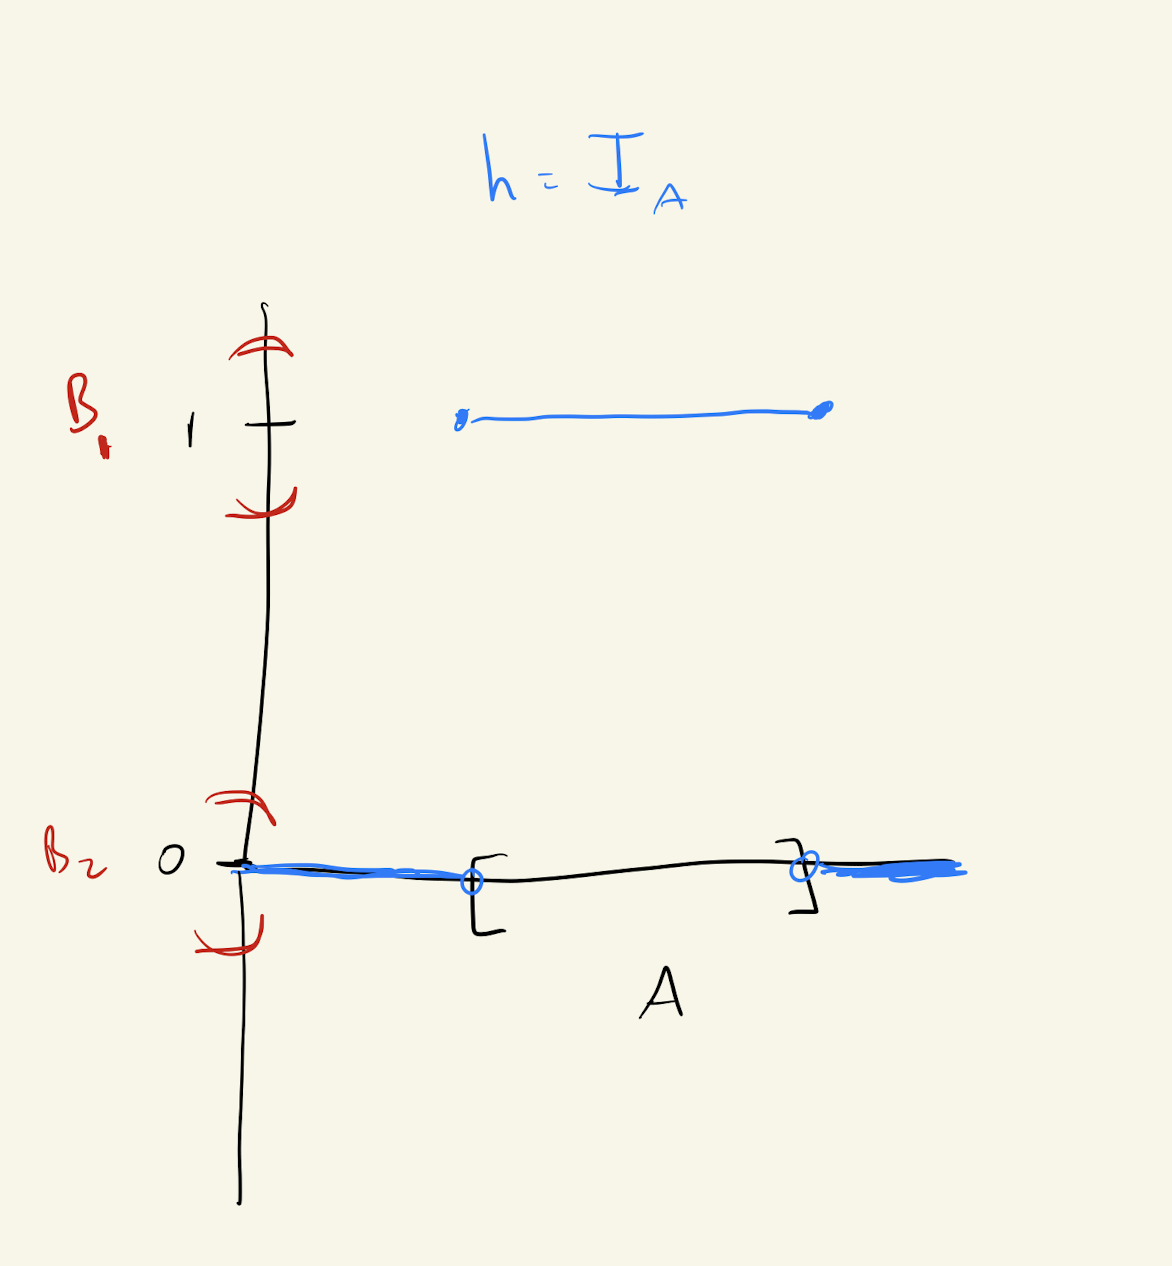
\includegraphics[width=.5\textwidth]{images/indicator_of_borel_set}	
\end{figure}

\end{example}

\begin{example}{\remarktitle{Indicators of non-Borel sets are not Borel measurable - but they may still be measurable.}}
Let $A$ be a subset of $\R$ that is not Borel (e.g., $A$ could be the non-Borel set described in Section \ref{sec:set_that_is_not_lesbesgue_measurable}), and let $I_A : \R \to \R$ be the indicator of $A$.   Then $I_A$ is \textit{not} Borel measurable.  

However, $I_A$  \textit{is} measurable with respect to the trivial sigma-field; that is, if we take the mapping to be $I_A : (\R, \B(\R)) \to (\R, \F_2)$, where $F_2 := \set{\emptyset, \R}$.  See Example \ref{ex:any_function_is_measurable_with_respect_to_trivial_sigma_field}.
\label{ex:indicators_of_non_borel_sets_are_not_borel_measurable}
\end{example}

\begin{example}{\remarktitle{Continuous functions are Borel measurable}}. Let $h : \R^k \to \R^n$ be continuous.  Since $h$ is continuous, the inverse image of any open set is open. Hence $h$ is Borel measurable by the computational definition of Borel measurability -- see Remark \ref{rk:computational_definition_of_Borel_measurability}.
\end{example}

\subsubsection{Why define measurability this way?}

Measurable functions do \textit{not} preserve measurability in \textit{both} directions. That is, if $h : (\Omega_1, \F_1) \to (\Omega_2, \F_2)$ is a measurable function, it is not necessarily true that $h(A) \in \F_2$ for all $A \in \F_1$.  For a counterexample, we take $\F_2 = \set{\emptyset, \Omega_2}$, recalling Example \ref{ex:any_function_is_measurable_with_respect_to_trivial_sigma_field}.   Then any $h$ is measurable.  But if $h(A)$ is a nonempty proper subset of $\Omega_2$, then it is not a measurable set, and so $h$ will not be measurable. 

So why is measurability defined by preserving measurability over \textit{inverse} images, rather than in terms of direct images?  In measure theory, inverse images are much nicer objects than direct images.  This is because basic set operations are preserved by inverse images, but in general not by images.  

In particular, for any function $f$
\begin{alphabate}
\item Inverse images and complements commute: $f^{-1}(B^c) = \big(f^{-1}(B)\big)^c$	

\textit{Proof.} $ \big(f^{-1}(B)\big)^c := \set{x : x \not\in f^{-1}(B) } = \set{x : f(x) \not\in B } = \set{x: f(x) \in B^c} = \set{x: x \in f^{-1}(B^c)} := f^{-1}(B^c).$

\item Inverse images and unions commute: $f^{-1}(\cup_i B_i) = \cup_i \big(f^{-1}(B_i)\big)$
\item Inverse images and intersections commute: $f^{-1}(\cap_i B_i) = \cap_i \big(f^{-1}(B_i)\big)$	
\end{alphabate}

However, 
\begin{itemize}
\item[d)] Direct images and complements do not in general commute: $f(A^c) \neq \big(f(A)\big)^c$	

\textit{Proof.} Let $f : \Omega \to \R$ be the constant function, i.e. $f(\omega) = c$ for some $c \in \R$ for all $\omega \in \Omega$.  Let $A$ be a non-empty proper subset of $\Omega$.  Then $h(A) = c$ and $h(A^c) = c$.  So $\R \setminus c = \big(h(A)\big)^c \neq  h(A^c) = c$.

\begin{figure}[H]
\centering
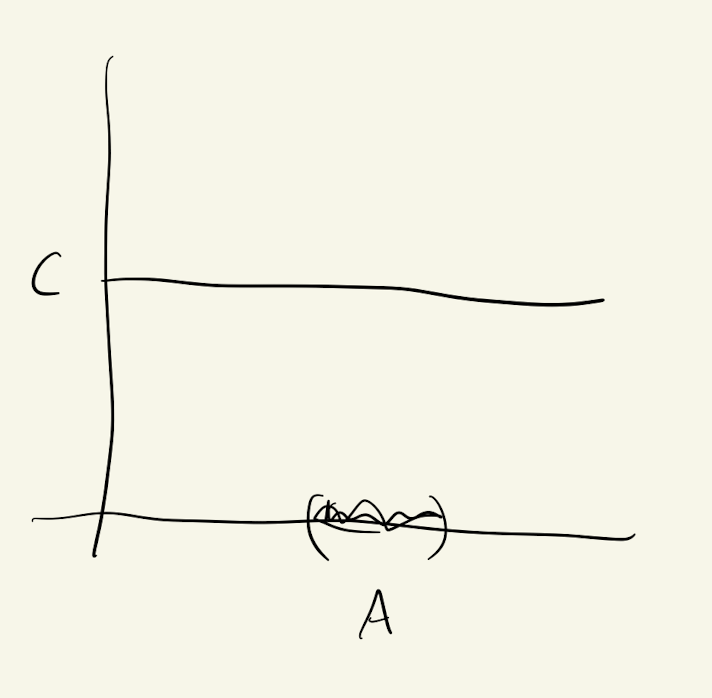
\includegraphics[width=.25\textwidth]{images/direct_images_and_complements}	
\end{figure}


\item[e)] Direct images and intersections do not in general commute: $f(\cap_i A_i) \neq \cap_i \big(f(A_i)\big)$	
\end{itemize}

Recall in Section \ref{sec:intuition_on_lesbesgue_integration} that Lesbesgue and Reimann integration are distinguished in terms of whether they partition the range or domain of the function.  My speculation is that the nice interplay of basic set operations and inverse images (but not direct images) at least partially explains why Lesbesgue's approach has been more successful than Reimann's approach (in the sense of better limit theorems, better handling of non-Euclidean spaces, etc.).

\subsection{$\S$ 1.5.2-1.5.3 Definition of the integral for Borel measurable functions}

In this section, we define integral of a Borel measurable function $h : (\Omega, \F) \to (\overline{\R}, \B(\overline{\R}))$ against arbitrary measure $\mu$.  The integral can be written as:
\[ \ds\int_{\Omega} h \wrt{\mu}, \quad \quad \ds\int_{\Omega} h(\omega) \wrt{\mu(\omega)}, \quad \text{ or } \quad \ds\int_{\Omega} h(\omega) \mu(d \, \omega) \]
 
 We proceed in three steps: first, we consider where $h$ is simple, then we consider $h$ non-negative, then we consider $h$ arbitrary. 

\subsubsection{Integrals of simple functions}

First we define simple functions. 

\begin{definition}
Let $(\Omega, \F)$ be a measurable space, fixed throughout the discussion.  If $h : \Omega \to \overline{\R}$, $h$ is said to be \textit{simple} iff $h$ is measurable and takes on only finitely many distinct values.  That is, $h$ is simple iff it can be written $h = \sum_{i=1}^r y_i I_{A_i}$ where the $A_i$ are disjoint sets in $\F$ and $I_{A_i}$ is the indicator of $A_i$; the $y_i$ need not be distinct. 
\label{def:simple_function}	
\end{definition}

\begin{remark}{\remarktitle{Simple functions generalize step functions}}
A special case of simple functions are the step functions used in Reimann integration. 


For $a,b \in \overline{\R}$ with $a<b$, $f : [a,b] \to \R$ is a \textit{step function} if there exists a partition $a = x_0 < x_1 < ... < x_n = b$ and constants $y_1, ..., y_n \in \R$ such that $f(x)=y_i$ for all $y \in (x_{i-1},x_i)$ and each $i=1,...,n$.  Then $f$ is equal to the following simple function:
\[ y_i I_{(x_{i-1}, x_i)} + f(x_i) I_{\set{x_i}}\]

Some observations:
\begin{itemize}
\item In this case, the sets $A_i$ take on a specific form, as open intervals or singletons.  In general, simple functions allow more general $A_i$. 
\item Simple functions do not require that the domain is totally ordered.  
\end{itemize}
\label{rk:simple_functions_generalize_step_functions}
\end{remark}

\begin{remark}
Note that the indicator function for a non-Borel set (see Example \ref{ex:indicators_of_non_borel_sets_are_not_borel_measurable}) is \textit{not} a simple function, even though it only takes on values 0 and 1. 
%Note that the term \textit{simple} in simple function refers to properties of \textit{both} the domain and range. So for instance, the indicator function for a non-Borel set (see Example \ref{ex:indicators_of_non_borel_sets_are_not_borel_measurable}) is \textit{not} a simple function, even though it only takes on values 0 and 1.  
\end{remark}

\paragraph{Definition of the integral of simple functions}

\begin{definition}
Let $h$ be simple, say $h = \sum_{i=1}^r y_i I_{A_i}$ where the $A_i$ are disjoint sets in $\F$.  Then
\begin{align*}
\ds\int_{\Omega} h \wrt{\mu} := \ds\sum_{i=1}^r y_i I_{A_i}.
\labelit \label{eqn:integral_of_simple_function}	
\end{align*}
 \label{def:integral_of_simple_function}
\end{definition}

The integral of a simple function can also be expressed as 
\[\ds\int_{\Omega} h \wrt{\mu} := \ds\sum_{i=1}^r y_i \; \mu \bigg( h^{-1}(y_i) \bigg) \]

\begin{figure}[H]
\centering 
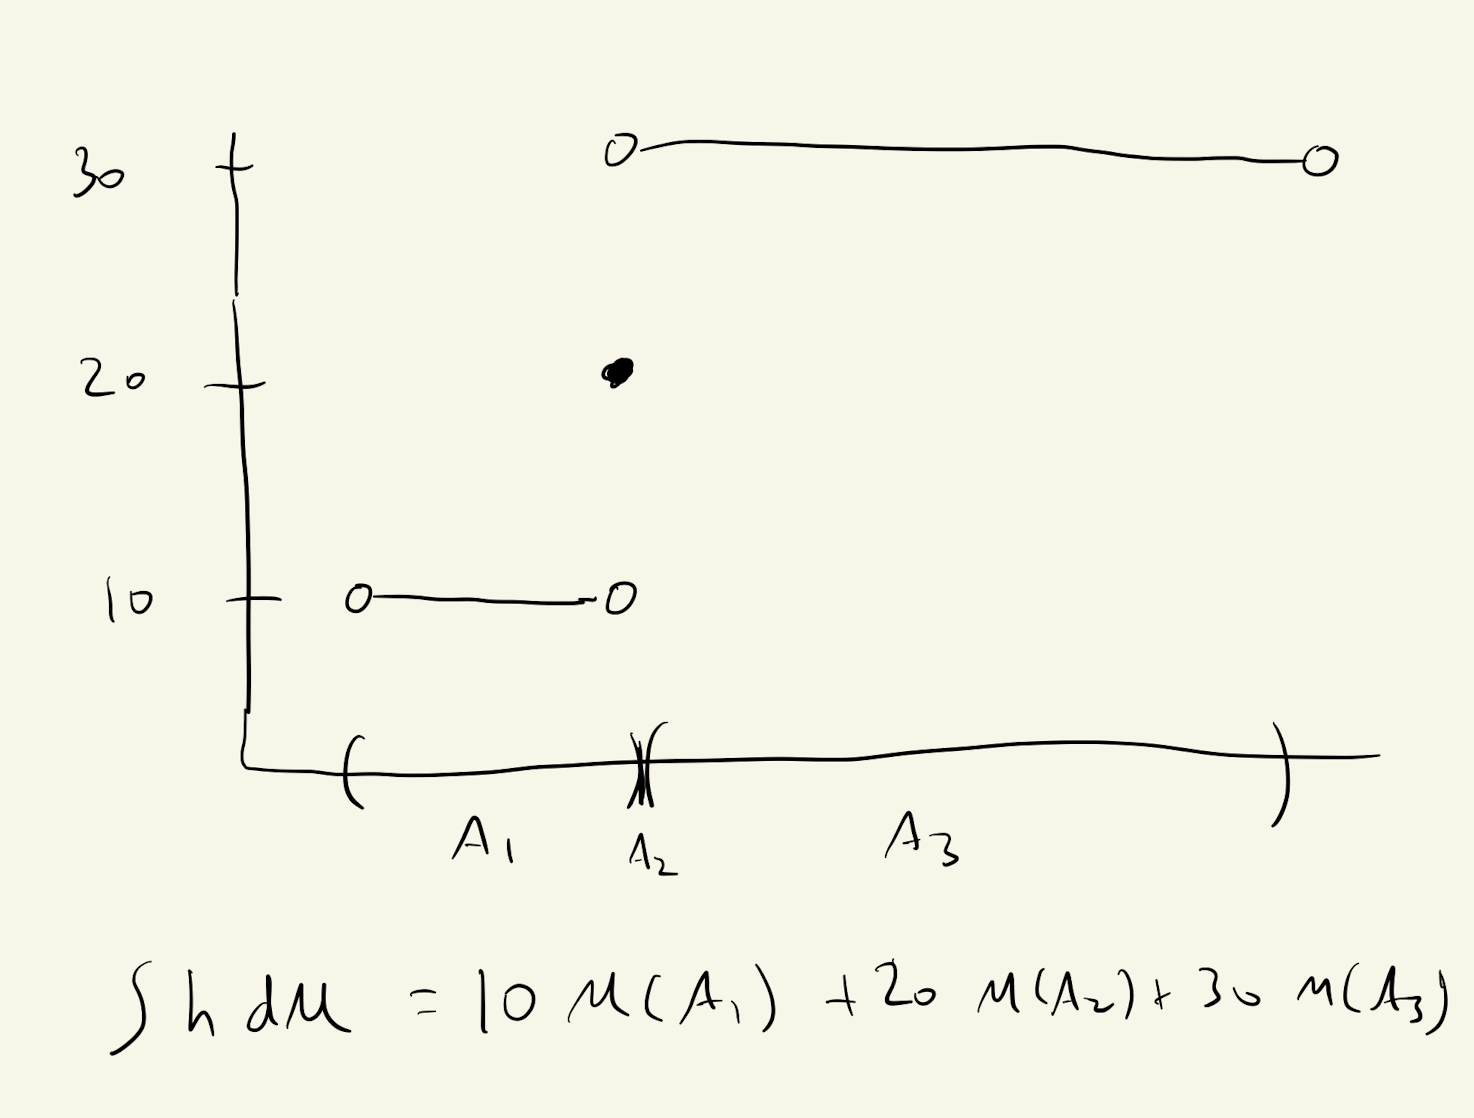
\includegraphics[width=.5\textwidth]{images/integral_of_simple_function}	
\caption{The Lesbesgue integral of a simple function. {\scriptsize (In this case, the simple function is also a step function.)}}
\end{figure}

\begin{example}{\remarktitle{Integrating a step function}}
Let $h$ be a step function, as defined in Remark \ref{rk:simple_functions_generalize_step_functions}.   So  $a = x_0 < x_1 < ... < x_n = b$ is a partition of $\Omega := \text{dom}(h)$, and $h$ takes on values $y_i$ on $(x_{i-1},x_i)$ for $i=1,...,n$.  Then 
\begin{align*}
\ds\int_{\Omega} h \wrt{\mu} &= \ds\sum_{i=1}^n y_i \; \mu(x_{i-1},x_i) + \cancelto{0}{\ds\sum_{i=1}^n f(x_i) \mu\set{x_i}} \\
& \stackreltext{(if $\mu$ is Lesbesgue measure)}{=} \; \ds\sum_{i=1}^n y_i \; (x_i - x_{i-1})
\end{align*}

So the Lesbesgue integral of the step function agrees with the Reimann integral when $\mu$ is Lesbesgue measure (although not for general measure).
\end{example}

Now we turn to the integral of a simple function that is not a step function.

\begin{example}{\remarktitle{Integrating the Dirichlet function}}
Let $h$ be the Dirichlet function; that is $h = I_{\Q} : \R \to \R$ is the indicator of the rationals.  Let us integrate $h$ against Lesbesgue measure $\mu$. 
\begin{align*}
\ds\int_{\Omega} h \wrt{\mu} &= 1 \mu(\Q) && \tinytext{def. integral} \\
 	&= 1 \; \mu(\bigcupdot_{q \in \Q} \set{q}) && \tinytext{rewrite $\Q$} \\
&= 1 \; \ds\sum_{q \in \Q} \mu(\set{q}) && \tinytext{countable additivity, $\Q$ is countable} \\
& \stackrel{1}{=} 1 \ds\sum_{q \in \Q} 0 && \tinytext{Proposition \ref{prop:properties_of_LS_measures}s} \\
&= 0.  
\end{align*}
Note Equation 1 holds for any Lesbesgue-Stieljes measure with a continuous distribution function (see Remark \ref{rk:continuity_at_a_point_iffi_measure_zero_at_a_point}).  However, other measures may yield other results.
\end{example}






\bibliography{references_ash_notes.bib}
\bibliographystyle{unsrt}

\newpage 
\appendix

\section{Supremum and Infimum}

Following are some definitions and propositions that we use in the notes.\footnote{For a nice introductory overview, see \href{https://www.math.ucdavis.edu/~hunter/m125b/ch2.pdf}.}

First, we define upper and lower bounds.
\begin{definition}
A set $A \subset \R$ of real numbers is bounded from above if there exists a real number $M \in \R$, called an \textit{upper bound} of $A$, such that $x \leq M$ for every $x \in A$.  Similarly, $A$  is bounded from below if there exists a real number $m \in \R$, called an \textit{lower bound} of $A$, such that $x \geq m$ for every $x \in A$.  A set is \textit{bounded} if it is bounded from above and below.
\label{def:upper_and_lower_bound}	
\end{definition}


Now, we define infimum and supremum.
\begin{definition}
Suppose that $A \subset \R$ is a set of real numbers. If $M \in \R$ is an upper bound of $A$ such that $M \leq M'$ for every upper bound $M'$ of $A$, then $M$ is called the \textit{supremum} of $A$, denoted $M=\sup A$.   Similarly, if $m \in \R$ is an lower bound of $A$ such that $m \geq m'$ for every lower bound $m'$ of $A$, then $m$ is called the \textit{infimum} of $A$, denoted $m=\inf A$.\label{def:supremum_and_infimum}	
\end{definition}

We sometimes use an alternate characterization of infimum and supremum.

\begin{proposition}

If $A \subset \R$, then $M = \sup A$ if and only if (a) $M$ is an upper bound of $A$; (b) for every $M' < M$, there exists an $a \in A$ such that $a>M'$.  Similarly, $m = \inf A$ if and only if (a) $m$ is a lower bound of $A$; (b) for all $m'>m$, there exists an $a \in A$ such that $a<m'$.

\begin{proof}
We prove the alternate characterization for the supremum only, as the proof for infimum is similar.    We only need to show equivalence for the part (b)'s, as the part (a)'s are identical. 

We first show that the definition implies part the proposition.  We proceed by way of contradiction.  Let $M = \sup A$, $M' <M$, and suppose there is no $a \in A : a > M'$. Then $M'$ is an upper bound of $A$ where $M' <M$, contradicting part (b) of the definition of supremum.   

Now we show that the proposition implies the definition. Part (b) of the proposition implies that if $M' < M$, then $M'$ is not an upper bound. Thus part (b) of the definition is satisfied.
\end{proof}
\label{prop:supremum_and_infimum_alternate_characterization}
\end{proposition}



\begin{remark}
The (b) statement in Proposition \ref{prop:supremum_and_infimum_alternate_characterization} roughly tell us that any other candidate for a smaller supremum fails, because it will not be an upper bound.  Similarly, any other candidate for a larger infimum fails, because it will not be a lower bound. 	
\end{remark}

\begin{remark}
Another way to write Proposition \ref{prop:supremum_and_infimum_alternate_characterization} is as follows:	

If $A \subset \R$, then $M = \sup A$ if and only if (a) $M$ is an upper bound of $A$; (b) for all $\epsilon >0$, there exists an $a \in A$ such that $a>M-\epsilon$.  Similarly, $m = \inf A$ if and only if (a) $m$ is a lower bound of $A$; (b) for all $\epsilon >0$, there exists an $a \in A$ such that $a<m+\epsilon$.
\label{rk:usage_of_alternate_characterization_of_inf_and_sup}
\end{remark}





The proposition below characterizes the behavior of the infimum and supremum under set containment

\begin{proposition}
Suppose that $A$ and $B$ are subsets of $\R$ such that $A \subset B$.  If $\sup A$ and $\sup B$ exist, then $\sup A \leq \sup B$.  If $\inf A$ and $\inf B$ exist, then $\inf A \geq \inf B$.
\label{prop:sup_and_inf_for_subsets_are_tighter}
\end{proposition}

Now we characterize the behavior of infimum and supremum over set (Minskowski) sums and differences.

\begin{definition}
If $A, B \subset \R$ are non-empty, we define the \textit{Minkowski sum} of the two sets, denoted $A+B$, by 
\[ A + B := \set{z : z = x + y \text{ for some } x \in A, y \in B } \]
Similarly, we define the \textit{Minkowski difference} of two sets, denoted $A-B$, by
\[ A - B := \set{z : z = x - y \text{ for some } x \in A, y \in B } \]
\label{def:minkowski_sum_and_difference}	
\end{definition}

\begin{proposition}
If $A, B \subset \R$ are non-empty, then 
\begin{align*}
\sup (A+B) = \sup A + \sup B, &\quad \inf (A+B) = \inf A + \inf B 	 \\
\sup (A-B) = \sup A - \inf B, &\quad \inf (A-B) = \inf A - \sup B 	 \\
\end{align*}

\label{prop:sup_and_inf_for_minkowski_sum_and_diff}	
\end{proposition}

\begin{remark}
Proposition \ref{prop:sup_and_inf_for_minkowski_sum_and_diff} can be informally described as saying that the infimum and supremum distribute over addition and subtraction, but negative signs ``flip" infima to suprema, and vice versa. 
\end{remark}


\section{Miscellaneous}
\subsection{Right semi-closed intervals}
\begin{definition}
A \textbf{right semi-closed interval} is a set of the form $(a,b] = \set{x : a < x \leq b}, -\infty \leq a < b < \infty$.  By convention, we also count $(a,\infty)$ as right semi-closed for $-\infty \leq a < \infty$. 
\label{def:rsc_intervals}
\end{definition}

\subsection{DeMorgan's Law applies to relative complements} 

\begin{remark}
DeMorgan's Law also holds for relative complements.  That is, given a sequence of sets $A_1, A_2, ...$ that are subsets of another set $X$, we have:

\begin{align*}
X - \bigcap_{n=1}^\infty A_n = \bigcup_{n=1}^\infty (X - A_n)
\labelit \label{eqn:demorgan_for_relative_complements}	
\end{align*}

	
\end{remark}


\end{document}
